% Options for packages loaded elsewhere
\PassOptionsToPackage{unicode}{hyperref}
\PassOptionsToPackage{hyphens}{url}
\PassOptionsToPackage{dvipsnames,svgnames,x11names}{xcolor}
%
\documentclass[
  letterpaper,
  DIV=11,
  numbers=noendperiod]{scrartcl}

\usepackage{amsmath,amssymb}
\usepackage{iftex}
\ifPDFTeX
  \usepackage[T1]{fontenc}
  \usepackage[utf8]{inputenc}
  \usepackage{textcomp} % provide euro and other symbols
\else % if luatex or xetex
  \usepackage{unicode-math}
  \defaultfontfeatures{Scale=MatchLowercase}
  \defaultfontfeatures[\rmfamily]{Ligatures=TeX,Scale=1}
\fi
\usepackage{lmodern}
\ifPDFTeX\else  
    % xetex/luatex font selection
\fi
% Use upquote if available, for straight quotes in verbatim environments
\IfFileExists{upquote.sty}{\usepackage{upquote}}{}
\IfFileExists{microtype.sty}{% use microtype if available
  \usepackage[]{microtype}
  \UseMicrotypeSet[protrusion]{basicmath} % disable protrusion for tt fonts
}{}
\makeatletter
\@ifundefined{KOMAClassName}{% if non-KOMA class
  \IfFileExists{parskip.sty}{%
    \usepackage{parskip}
  }{% else
    \setlength{\parindent}{0pt}
    \setlength{\parskip}{6pt plus 2pt minus 1pt}}
}{% if KOMA class
  \KOMAoptions{parskip=half}}
\makeatother
\usepackage{xcolor}
\setlength{\emergencystretch}{3em} % prevent overfull lines
\setcounter{secnumdepth}{-\maxdimen} % remove section numbering
% Make \paragraph and \subparagraph free-standing
\makeatletter
\ifx\paragraph\undefined\else
  \let\oldparagraph\paragraph
  \renewcommand{\paragraph}{
    \@ifstar
      \xxxParagraphStar
      \xxxParagraphNoStar
  }
  \newcommand{\xxxParagraphStar}[1]{\oldparagraph*{#1}\mbox{}}
  \newcommand{\xxxParagraphNoStar}[1]{\oldparagraph{#1}\mbox{}}
\fi
\ifx\subparagraph\undefined\else
  \let\oldsubparagraph\subparagraph
  \renewcommand{\subparagraph}{
    \@ifstar
      \xxxSubParagraphStar
      \xxxSubParagraphNoStar
  }
  \newcommand{\xxxSubParagraphStar}[1]{\oldsubparagraph*{#1}\mbox{}}
  \newcommand{\xxxSubParagraphNoStar}[1]{\oldsubparagraph{#1}\mbox{}}
\fi
\makeatother

\usepackage{color}
\usepackage{fancyvrb}
\newcommand{\VerbBar}{|}
\newcommand{\VERB}{\Verb[commandchars=\\\{\}]}
\DefineVerbatimEnvironment{Highlighting}{Verbatim}{commandchars=\\\{\}}
% Add ',fontsize=\small' for more characters per line
\usepackage{framed}
\definecolor{shadecolor}{RGB}{241,243,245}
\newenvironment{Shaded}{\begin{snugshade}}{\end{snugshade}}
\newcommand{\AlertTok}[1]{\textcolor[rgb]{0.68,0.00,0.00}{#1}}
\newcommand{\AnnotationTok}[1]{\textcolor[rgb]{0.37,0.37,0.37}{#1}}
\newcommand{\AttributeTok}[1]{\textcolor[rgb]{0.40,0.45,0.13}{#1}}
\newcommand{\BaseNTok}[1]{\textcolor[rgb]{0.68,0.00,0.00}{#1}}
\newcommand{\BuiltInTok}[1]{\textcolor[rgb]{0.00,0.23,0.31}{#1}}
\newcommand{\CharTok}[1]{\textcolor[rgb]{0.13,0.47,0.30}{#1}}
\newcommand{\CommentTok}[1]{\textcolor[rgb]{0.37,0.37,0.37}{#1}}
\newcommand{\CommentVarTok}[1]{\textcolor[rgb]{0.37,0.37,0.37}{\textit{#1}}}
\newcommand{\ConstantTok}[1]{\textcolor[rgb]{0.56,0.35,0.01}{#1}}
\newcommand{\ControlFlowTok}[1]{\textcolor[rgb]{0.00,0.23,0.31}{\textbf{#1}}}
\newcommand{\DataTypeTok}[1]{\textcolor[rgb]{0.68,0.00,0.00}{#1}}
\newcommand{\DecValTok}[1]{\textcolor[rgb]{0.68,0.00,0.00}{#1}}
\newcommand{\DocumentationTok}[1]{\textcolor[rgb]{0.37,0.37,0.37}{\textit{#1}}}
\newcommand{\ErrorTok}[1]{\textcolor[rgb]{0.68,0.00,0.00}{#1}}
\newcommand{\ExtensionTok}[1]{\textcolor[rgb]{0.00,0.23,0.31}{#1}}
\newcommand{\FloatTok}[1]{\textcolor[rgb]{0.68,0.00,0.00}{#1}}
\newcommand{\FunctionTok}[1]{\textcolor[rgb]{0.28,0.35,0.67}{#1}}
\newcommand{\ImportTok}[1]{\textcolor[rgb]{0.00,0.46,0.62}{#1}}
\newcommand{\InformationTok}[1]{\textcolor[rgb]{0.37,0.37,0.37}{#1}}
\newcommand{\KeywordTok}[1]{\textcolor[rgb]{0.00,0.23,0.31}{\textbf{#1}}}
\newcommand{\NormalTok}[1]{\textcolor[rgb]{0.00,0.23,0.31}{#1}}
\newcommand{\OperatorTok}[1]{\textcolor[rgb]{0.37,0.37,0.37}{#1}}
\newcommand{\OtherTok}[1]{\textcolor[rgb]{0.00,0.23,0.31}{#1}}
\newcommand{\PreprocessorTok}[1]{\textcolor[rgb]{0.68,0.00,0.00}{#1}}
\newcommand{\RegionMarkerTok}[1]{\textcolor[rgb]{0.00,0.23,0.31}{#1}}
\newcommand{\SpecialCharTok}[1]{\textcolor[rgb]{0.37,0.37,0.37}{#1}}
\newcommand{\SpecialStringTok}[1]{\textcolor[rgb]{0.13,0.47,0.30}{#1}}
\newcommand{\StringTok}[1]{\textcolor[rgb]{0.13,0.47,0.30}{#1}}
\newcommand{\VariableTok}[1]{\textcolor[rgb]{0.07,0.07,0.07}{#1}}
\newcommand{\VerbatimStringTok}[1]{\textcolor[rgb]{0.13,0.47,0.30}{#1}}
\newcommand{\WarningTok}[1]{\textcolor[rgb]{0.37,0.37,0.37}{\textit{#1}}}

\providecommand{\tightlist}{%
  \setlength{\itemsep}{0pt}\setlength{\parskip}{0pt}}\usepackage{longtable,booktabs,array}
\usepackage{calc} % for calculating minipage widths
% Correct order of tables after \paragraph or \subparagraph
\usepackage{etoolbox}
\makeatletter
\patchcmd\longtable{\par}{\if@noskipsec\mbox{}\fi\par}{}{}
\makeatother
% Allow footnotes in longtable head/foot
\IfFileExists{footnotehyper.sty}{\usepackage{footnotehyper}}{\usepackage{footnote}}
\makesavenoteenv{longtable}
\usepackage{graphicx}
\makeatletter
\def\maxwidth{\ifdim\Gin@nat@width>\linewidth\linewidth\else\Gin@nat@width\fi}
\def\maxheight{\ifdim\Gin@nat@height>\textheight\textheight\else\Gin@nat@height\fi}
\makeatother
% Scale images if necessary, so that they will not overflow the page
% margins by default, and it is still possible to overwrite the defaults
% using explicit options in \includegraphics[width, height, ...]{}
\setkeys{Gin}{width=\maxwidth,height=\maxheight,keepaspectratio}
% Set default figure placement to htbp
\makeatletter
\def\fps@figure{htbp}
\makeatother

\usepackage{fvextra}
\DefineVerbatimEnvironment{Highlighting}{Verbatim}{breaklines,commandchars=\\\{\}}
\KOMAoption{captions}{tableheading}
\makeatletter
\@ifpackageloaded{caption}{}{\usepackage{caption}}
\AtBeginDocument{%
\ifdefined\contentsname
  \renewcommand*\contentsname{Table of contents}
\else
  \newcommand\contentsname{Table of contents}
\fi
\ifdefined\listfigurename
  \renewcommand*\listfigurename{List of Figures}
\else
  \newcommand\listfigurename{List of Figures}
\fi
\ifdefined\listtablename
  \renewcommand*\listtablename{List of Tables}
\else
  \newcommand\listtablename{List of Tables}
\fi
\ifdefined\figurename
  \renewcommand*\figurename{Figure}
\else
  \newcommand\figurename{Figure}
\fi
\ifdefined\tablename
  \renewcommand*\tablename{Table}
\else
  \newcommand\tablename{Table}
\fi
}
\@ifpackageloaded{float}{}{\usepackage{float}}
\floatstyle{ruled}
\@ifundefined{c@chapter}{\newfloat{codelisting}{h}{lop}}{\newfloat{codelisting}{h}{lop}[chapter]}
\floatname{codelisting}{Listing}
\newcommand*\listoflistings{\listof{codelisting}{List of Listings}}
\makeatother
\makeatletter
\makeatother
\makeatletter
\@ifpackageloaded{caption}{}{\usepackage{caption}}
\@ifpackageloaded{subcaption}{}{\usepackage{subcaption}}
\makeatother

\ifLuaTeX
  \usepackage{selnolig}  % disable illegal ligatures
\fi
\usepackage{bookmark}

\IfFileExists{xurl.sty}{\usepackage{xurl}}{} % add URL line breaks if available
\urlstyle{same} % disable monospaced font for URLs
\hypersetup{
  pdftitle={Problem Set 4},
  colorlinks=true,
  linkcolor={blue},
  filecolor={Maroon},
  citecolor={Blue},
  urlcolor={Blue},
  pdfcreator={LaTeX via pandoc}}


\title{Problem Set 4}
\author{}
\date{}

\begin{document}
\maketitle

\RecustomVerbatimEnvironment{verbatim}{Verbatim}{
  showspaces = false,
  showtabs = false,
  breaksymbolleft={},
  breaklines
}


\textbf{PS4:} Due Sat Nov 2 at 5:00PM Central. Worth 100 points. We use
(\texttt{*}) to indicate a problem that we think might be time
consuming.

\subsection{Style Points (10 pts)}\label{style-points-10-pts}

Please refer to the minilesson on code style
\textbf{\href{https://uchicago.zoom.us/rec/share/pG_wQ-pHTQrJTmqNn4rcrw5V194M2H2s-2jdy8oVhWHkd_yZt9o162IWurpA-fxU.BIQlSgZLRYctvzp-}{here}}.

\subsection{Submission Steps (10 pts)}\label{submission-steps-10-pts}

\begin{enumerate}
\def\labelenumi{\arabic{enumi}.}
\tightlist
\item
  This problem set is a paired problem set.
\item
  Play paper, scissors, rock to determine who goes first. Call that
  person \emph{Partner 1}.

  \begin{itemize}
  \tightlist
  \item
    Partner 1 : Sijie Wu, sijiewu
  \item
    Partner 2 : Abu Bakar Siddique, abubakars
  \end{itemize}
\item
  Partner 1 will accept the \texttt{ps4} and then share the link it
  creates with their partner. You can only share it with one partner so
  you will not be able to change it after your partner has accepted.
\item
  ``This submission is our work alone and complies with the 30538
  integrity policy.'' Add your initials to indicate your agreement:
  **\_\_** **\_\_**
\item
  ``I have uploaded the names of anyone else other than my partner and I
  worked with on the problem set
  \textbf{\href{https://docs.google.com/forms/d/185usrCREQaUbvAXpWhChkjghdGgmAZXA3lPWpXLLsts/edit}{here}}''
  (1 point)
\item
  Late coins used this pset: **\_\_** Late coins left after submission:
  **\_\_**
\item
  Knit your \texttt{ps4.qmd} to an PDF file to make \texttt{ps4.pdf},

  \begin{itemize}
  \tightlist
  \item
    The PDF should not be more than 25 pages. Use \texttt{head()} and
    re-size figures when appropriate.
  \end{itemize}
\item
  (Partner 1): push \texttt{ps4.qmd} and \texttt{ps4.pdf} to your github
  repo.
\item
  (Partner 1): submit \texttt{ps4.pdf} via Gradescope. Add your partner
  on Gradescope.
\item
  (Partner 1): tag your submission in Gradescope
\end{enumerate}

\textbf{Important:} Repositories are for tracking code. \textbf{Do not
commit the data or shapefiles to your repo.} The best way to do this is
with \texttt{.gitignore}, which we have covered in class. If you do
accidentally commit the data, Github has a
\href{https://docs.github.com/en/repositories/working-with-files/managing-large-files/about-large-files-on-github\#removing-files-from-a-repositorys-history}{guide}.
The best course of action depends on whether you have pushed yet. This
also means that both partners will have to download the initial raw data
and any data cleaning code will need to be re-run on both partners'
computers.

\subsection{Download and explore the Provider of Services (POS) file (10
pts)}\label{download-and-explore-the-provider-of-services-pos-file-10-pts}

\begin{enumerate}
\def\labelenumi{\arabic{enumi}.}
\item
  \texttt{PRVDR\_CTGRY\_SBTYP\_CD} for provider subtype code;
  \texttt{PRVDR\_CTGRY\_CD} for provider type code; \texttt{PRVDR\_NUM}
  for CMS Certification Number; \texttt{PGM\_TRMNTN\_CD} for Termination
  Code; \texttt{ZIP\_CD} for zip code; \texttt{TRMNTN\_EXPRTN\_DT} for
  Termination Date; \texttt{FAC\_NAME} for facility name.
\item
\end{enumerate}

\begin{Shaded}
\begin{Highlighting}[]
\ImportTok{import}\NormalTok{ pandas }\ImportTok{as}\NormalTok{ pd}
\NormalTok{filepath1 }\OperatorTok{=} \StringTok{"pos2016.csv"}
\NormalTok{pos2016 }\OperatorTok{=}\NormalTok{ pd.read\_csv(filepath1)}
\NormalTok{pos2016.head()}
\NormalTok{pos2016[}\StringTok{"year"}\NormalTok{] }\OperatorTok{=} \DecValTok{2016}
\NormalTok{pos2016\_short }\OperatorTok{=}\NormalTok{ pos2016[(pos2016[}\StringTok{"PRVDR\_CTGRY\_CD"}\NormalTok{] }\OperatorTok{==} \DecValTok{1}\NormalTok{) }\OperatorTok{\&}\NormalTok{ (pos2016[}\StringTok{"PRVDR\_CTGRY\_SBTYP\_CD"}\NormalTok{] }\OperatorTok{==} \DecValTok{1}\NormalTok{)]}
\end{Highlighting}
\end{Shaded}

\begin{Shaded}
\begin{Highlighting}[]
\NormalTok{unique\_count1 }\OperatorTok{=}\NormalTok{ pos2016\_short[}\StringTok{\textquotesingle{}FAC\_NAME\textquotesingle{}}\NormalTok{].nunique()}
\NormalTok{unique\_count2 }\OperatorTok{=}\NormalTok{ pos2016\_short[}\StringTok{\textquotesingle{}PRVDR\_NUM\textquotesingle{}}\NormalTok{].nunique()}
\BuiltInTok{print}\NormalTok{(}\SpecialStringTok{f"Number of unique PRVDR\_NUM values: }\SpecialCharTok{\{}\NormalTok{unique\_count2}\SpecialCharTok{\}}\SpecialStringTok{"}\NormalTok{)}
\BuiltInTok{print}\NormalTok{(}\SpecialStringTok{f"Number of unique FAC\_NAME values: }\SpecialCharTok{\{}\NormalTok{unique\_count1}\SpecialCharTok{\}}\SpecialStringTok{"}\NormalTok{)}
\end{Highlighting}
\end{Shaded}

\begin{verbatim}
Number of unique PRVDR_NUM values: 7245
Number of unique FAC_NAME values: 6770
\end{verbatim}

\begin{verbatim}
a. I use `FAC_NAME` and `PRVDR_NUM` respectively to calculate the unique value of the short-term hospitals. Under CMS Certification Number, there are 7245 unique hospitals in Q4 2016 data set. Under facility name, there are 6770 unique hospitals in Q4 2016 data set. I believe this number is a bit large for short-term hospitals in Q4 2016.

b. I searched for number of hospitals in 2020 to 2024 on [this website] (https://www.aha.org/statistics/fast-facts-us-hospitals), and discovers that the total number of hospitals in the United States is a little bit more than 6000, with 6039 in 2022 and 6120 in 2024. Also, [Kaiser Family Foundation] (https://www.kff.org/report-section/a-look-at-rural-hospital-closures-and-implications-for-access-to-care-three-case-studies-issue-brief/) states that, there are nearly 5000 short-term hospitals in the US.

I believe the reason behind the difference is that, some hospitals change names over the time, and even though using the unique value of `facility name`, the hospitals are still not unique.
\end{verbatim}

\begin{enumerate}
\def\labelenumi{\arabic{enumi}.}
\tightlist
\item
\end{enumerate}

\begin{Shaded}
\begin{Highlighting}[]
\NormalTok{filepath2 }\OperatorTok{=} \StringTok{"pos2017.csv"}
\NormalTok{pos2017 }\OperatorTok{=}\NormalTok{ pd.read\_csv(filepath2)}
\NormalTok{pos2017[}\StringTok{"year"}\NormalTok{] }\OperatorTok{=} \DecValTok{2017}
\NormalTok{pos2017\_short }\OperatorTok{=}\NormalTok{ pos2017[(pos2017[}\StringTok{"PRVDR\_CTGRY\_CD"}\NormalTok{] }\OperatorTok{==} \DecValTok{1}\NormalTok{) }\OperatorTok{\&}\NormalTok{ (pos2017[}\StringTok{"PRVDR\_CTGRY\_SBTYP\_CD"}\NormalTok{] }\OperatorTok{==} \DecValTok{1}\NormalTok{)]}


\NormalTok{filepath3 }\OperatorTok{=} \StringTok{"pos2018.csv"}
\NormalTok{pos2018 }\OperatorTok{=}\NormalTok{ pd.read\_csv(filepath3, encoding}\OperatorTok{=}\StringTok{\textquotesingle{}ISO{-}8859{-}1\textquotesingle{}}\NormalTok{)}
\NormalTok{pos2018[}\StringTok{"year"}\NormalTok{] }\OperatorTok{=} \DecValTok{2018}
\NormalTok{pos2018\_short }\OperatorTok{=}\NormalTok{ pos2018[(pos2018[}\StringTok{"PRVDR\_CTGRY\_CD"}\NormalTok{] }\OperatorTok{==} \DecValTok{1}\NormalTok{) }\OperatorTok{\&}\NormalTok{ (pos2018[}\StringTok{"PRVDR\_CTGRY\_SBTYP\_CD"}\NormalTok{] }\OperatorTok{==} \DecValTok{1}\NormalTok{)]}

\NormalTok{filepath4 }\OperatorTok{=} \StringTok{"pos2019.csv"}
\NormalTok{pos2019 }\OperatorTok{=}\NormalTok{ pd.read\_csv(filepath4, encoding}\OperatorTok{=}\StringTok{\textquotesingle{}ISO{-}8859{-}1\textquotesingle{}}\NormalTok{)}
\NormalTok{pos2019[}\StringTok{"year"}\NormalTok{] }\OperatorTok{=} \DecValTok{2019}
\NormalTok{pos2019\_short }\OperatorTok{=}\NormalTok{ pos2019[(pos2019[}\StringTok{"PRVDR\_CTGRY\_CD"}\NormalTok{] }\OperatorTok{==} \DecValTok{1}\NormalTok{) }\OperatorTok{\&}\NormalTok{ (pos2019[}\StringTok{"PRVDR\_CTGRY\_SBTYP\_CD"}\NormalTok{] }\OperatorTok{==} \DecValTok{1}\NormalTok{)]}
\end{Highlighting}
\end{Shaded}

\begin{Shaded}
\begin{Highlighting}[]
\NormalTok{pos\_merge }\OperatorTok{=}\NormalTok{ pd.concat([pos2016\_short, pos2017\_short, pos2018\_short, pos2019\_short], ignore\_index}\OperatorTok{=}\VariableTok{True}\NormalTok{)}
\NormalTok{pos\_merge.shape}
\NormalTok{pos\_merge.to\_csv(}\StringTok{"pos\_merge.csv"}\NormalTok{, index }\OperatorTok{=} \VariableTok{False}\NormalTok{)}
\end{Highlighting}
\end{Shaded}

The plot of number of observations by year is as followed.

\begin{Shaded}
\begin{Highlighting}[]
\ImportTok{import}\NormalTok{ altair }\ImportTok{as}\NormalTok{ alt}
\ImportTok{from}\NormalTok{ altair\_saver }\ImportTok{import}\NormalTok{ save}

\NormalTok{year\_count }\OperatorTok{=}\NormalTok{ pos\_merge[}\StringTok{"year"}\NormalTok{].value\_counts().reset\_index()}
\NormalTok{year\_count.columns }\OperatorTok{=}\NormalTok{ [}\StringTok{"year"}\NormalTok{, }\StringTok{"count"}\NormalTok{]}

\NormalTok{chart1 }\OperatorTok{=}\NormalTok{ alt.Chart(year\_count).mark\_bar().encode(}
\NormalTok{    x }\OperatorTok{=}\NormalTok{ alt.X(}\StringTok{"count:Q"}\NormalTok{, title }\OperatorTok{=} \StringTok{"Number of Observations"}\NormalTok{),}
\NormalTok{    y }\OperatorTok{=}\NormalTok{ alt.Y(}\StringTok{"year:N"}\NormalTok{, title }\OperatorTok{=} \StringTok{"year"}\NormalTok{)}
\NormalTok{).properties(}
\NormalTok{    title }\OperatorTok{=} \StringTok{"Number of Observations by Year"}
\NormalTok{)}

\CommentTok{\#save(chart1, \textquotesingle{}chart1.png\textquotesingle{})}
\end{Highlighting}
\end{Shaded}

\begin{figure}[H]

{\centering \includegraphics{chart1.png}

}

\caption{Number of Observations by Year}

\end{figure}%

\begin{enumerate}
\def\labelenumi{\arabic{enumi}.}
\tightlist
\item
  \begin{enumerate}
  \def\labelenumii{\alph{enumii}.}
  \tightlist
  \item
  \end{enumerate}
\end{enumerate}

\begin{Shaded}
\begin{Highlighting}[]
\NormalTok{year\_count\_unique }\OperatorTok{=}\NormalTok{ pos\_merge.groupby(}
    \StringTok{"year"}\NormalTok{)[}\StringTok{"PRVDR\_NUM"}\NormalTok{].nunique().reset\_index()}
\NormalTok{year\_count\_unique.columns }\OperatorTok{=}\NormalTok{ [}\StringTok{"year"}\NormalTok{, }\StringTok{"count"}\NormalTok{]}

\NormalTok{chart2 }\OperatorTok{=}\NormalTok{ alt.Chart(year\_count\_unique).mark\_bar().encode(}
\NormalTok{    x}\OperatorTok{=}\NormalTok{alt.X(}\StringTok{"count:Q"}\NormalTok{, title}\OperatorTok{=}\StringTok{"Number of Hospitals"}\NormalTok{),}
\NormalTok{    y}\OperatorTok{=}\NormalTok{alt.Y(}\StringTok{"year:N"}\NormalTok{, title}\OperatorTok{=}\StringTok{"year"}\NormalTok{)}
\NormalTok{).properties(}
\NormalTok{    title}\OperatorTok{=}\StringTok{"Number of Unique Hospitals by Year"}
\NormalTok{)}

\CommentTok{\#chart2}
\end{Highlighting}
\end{Shaded}

\begin{figure}[H]

{\centering \includegraphics{chart2.png}

}

\caption{Number of Unique Hospitals by Year}

\end{figure}%

\begin{verbatim}
b.
\end{verbatim}

These two plots are the same. It means that the CMS certification number
corresponds uniquely with the observations of hospitals.

\subsection{Identify hospital closures in POS file (15 pts)
(*)}\label{identify-hospital-closures-in-pos-file-15-pts}

\begin{enumerate}
\def\labelenumi{\arabic{enumi}.}
\tightlist
\item
\end{enumerate}

\begin{Shaded}
\begin{Highlighting}[]
\NormalTok{hospital\_active2016 }\OperatorTok{=}\NormalTok{ pos2016\_short[pos2016\_short[}\StringTok{"PGM\_TRMNTN\_CD"}\NormalTok{] }\OperatorTok{==} \DecValTok{0}\NormalTok{][}\StringTok{"PRVDR\_NUM"}\NormalTok{].unique()}
\NormalTok{hospital\_close\_suspect }\OperatorTok{=}\NormalTok{ []}
\ControlFlowTok{for}\NormalTok{ hospital\_id }\KeywordTok{in}\NormalTok{ hospital\_active2016:}
\NormalTok{    hospital\_data }\OperatorTok{=}\NormalTok{ pos\_merge[pos\_merge[}\StringTok{"PRVDR\_NUM"}\NormalTok{] }\OperatorTok{==}\NormalTok{ hospital\_id].sort\_values(by}\OperatorTok{=}\StringTok{"year"}\NormalTok{)}
\NormalTok{    closed }\OperatorTok{=} \VariableTok{False}
    \ControlFlowTok{for}\NormalTok{ year }\KeywordTok{in} \BuiltInTok{range}\NormalTok{(}\DecValTok{2017}\NormalTok{, }\DecValTok{2020}\NormalTok{):  }\CommentTok{\# 2017 to 2019}
\NormalTok{        year\_data }\OperatorTok{=}\NormalTok{ hospital\_data[hospital\_data[}\StringTok{"year"}\NormalTok{] }\OperatorTok{==}\NormalTok{ year]}
        \ControlFlowTok{if}\NormalTok{ year\_data.empty }\KeywordTok{or}\NormalTok{ (year\_data[}\StringTok{"PGM\_TRMNTN\_CD"}\NormalTok{].iloc[}\DecValTok{0}\NormalTok{] }\OperatorTok{!=} \DecValTok{0}\NormalTok{):}
            \CommentTok{\# If hospital data is missing or not active in this year, record closure details}
\NormalTok{            facility\_name }\OperatorTok{=}\NormalTok{ hospital\_data[}\StringTok{"FAC\_NAME"}\NormalTok{].iloc[}\DecValTok{0}\NormalTok{]}
\NormalTok{            zip\_code }\OperatorTok{=}\NormalTok{ hospital\_data[}\StringTok{"ZIP\_CD"}\NormalTok{].iloc[}\DecValTok{0}\NormalTok{]}
\NormalTok{            hospital\_close\_suspect.append(\{}
                \StringTok{"PRVDR\_NUM"}\NormalTok{: hospital\_id,}
                \StringTok{"FAC\_NAME"}\NormalTok{: facility\_name,}
                \StringTok{"ZIP\_CD"}\NormalTok{: zip\_code,}
                \StringTok{"year"}\NormalTok{: year}
\NormalTok{            \})}
\NormalTok{            closed }\OperatorTok{=} \VariableTok{True}
            \ControlFlowTok{break} 

\NormalTok{hospital\_close\_suspect }\OperatorTok{=}\NormalTok{ pd.DataFrame(hospital\_close\_suspect)}
\end{Highlighting}
\end{Shaded}

There are 174 hospitals fit this definition.

\begin{enumerate}
\def\labelenumi{\arabic{enumi}.}
\setcounter{enumi}{1}
\tightlist
\item
\end{enumerate}

\begin{Shaded}
\begin{Highlighting}[]
\NormalTok{hospital\_close\_suspect }\OperatorTok{=}\NormalTok{ hospital\_close\_suspect.sort\_values(by }\OperatorTok{=} \StringTok{"FAC\_NAME"}\NormalTok{)}

\NormalTok{hospital\_close\_top\_10 }\OperatorTok{=}\NormalTok{ hospital\_close\_suspect[[}\StringTok{\textquotesingle{}FAC\_NAME\textquotesingle{}}\NormalTok{, }\StringTok{\textquotesingle{}year\textquotesingle{}}\NormalTok{]].head(}\DecValTok{10}\NormalTok{)}
\BuiltInTok{print}\NormalTok{(hospital\_close\_top\_10)}
\end{Highlighting}
\end{Shaded}

\begin{verbatim}
                                        FAC_NAME  year
0                         ABRAZO MARYVALE CAMPUS  2017
1      ADVENTIST MEDICAL CENTER - CENTRAL VALLEY  2017
2                        AFFINITY MEDICAL CENTER  2018
3  ALBANY MEDICAL CENTER / SOUTH CLINICAL CAMPUS  2017
4       ALLEGIANCE SPECIALTY HOSPITAL OF KILGORE  2017
5                        ALLIANCE LAIRD HOSPITAL  2019
6                       ALLIANCEHEALTH DEACONESS  2019
7                  ANNE BATES LEACH EYE HOSPITAL  2019
8        ARKANSAS VALLEY REGIONAL MEDICAL CENTER  2017
9            BANNER CHURCHILL COMMUNITY HOSPITAL  2017
\end{verbatim}

\begin{enumerate}
\def\labelenumi{\arabic{enumi}.}
\setcounter{enumi}{2}
\tightlist
\item
  I devide the question into two steps, and use GPT by asking 1) how to
  count the active hospitals by ZIP code for each year; and 2) how to
  identity the zip codes that the number of hospitals do not decrease in
  the next year.
\end{enumerate}

\begin{Shaded}
\begin{Highlighting}[]
\CommentTok{\# Step 1: Count active hospitals by ZIP code for each year (0 in PGM\_TRMNTN\_CD indicates "Active Provider")}
\NormalTok{active\_hospitals\_by\_zip }\OperatorTok{=}\NormalTok{ pos\_merge[pos\_merge[}\StringTok{"PGM\_TRMNTN\_CD"}\NormalTok{] }\OperatorTok{==} \DecValTok{0}\NormalTok{].groupby(}
\NormalTok{    [}\StringTok{"ZIP\_CD"}\NormalTok{, }\StringTok{"year"}\NormalTok{])[}\StringTok{"PRVDR\_NUM"}\NormalTok{].nunique().reset\_index()}
\NormalTok{active\_hospitals\_by\_zip.columns }\OperatorTok{=}\NormalTok{ [}\StringTok{"ZIP\_CD"}\NormalTok{, }\StringTok{"year"}\NormalTok{, }\StringTok{"active\_hospitals"}\NormalTok{]}

\CommentTok{\# Step 2: Identify ZIP codes to filter out}
\NormalTok{zip\_codes\_to\_filter }\OperatorTok{=}\NormalTok{ []}
\ControlFlowTok{for}\NormalTok{ \_, row }\KeywordTok{in}\NormalTok{ active\_hospitals\_by\_zip.iterrows():}
\NormalTok{    zip\_code }\OperatorTok{=}\NormalTok{ row[}\StringTok{"ZIP\_CD"}\NormalTok{]}
\NormalTok{    current\_year }\OperatorTok{=}\NormalTok{ row[}\StringTok{"year"}\NormalTok{]}
\NormalTok{    current\_count }\OperatorTok{=}\NormalTok{ row[}\StringTok{"active\_hospitals"}\NormalTok{]}

    \CommentTok{\# Get count for the following year}
\NormalTok{    next\_year\_data }\OperatorTok{=}\NormalTok{ active\_hospitals\_by\_zip[(active\_hospitals\_by\_zip[}\StringTok{"ZIP\_CD"}\NormalTok{] }\OperatorTok{==}\NormalTok{ zip\_code) }\OperatorTok{\&}
\NormalTok{                                             (active\_hospitals\_by\_zip[}\StringTok{"year"}\NormalTok{] }\OperatorTok{==}\NormalTok{ current\_year }\OperatorTok{+} \DecValTok{1}\NormalTok{)]}

    \ControlFlowTok{if} \KeywordTok{not}\NormalTok{ next\_year\_data.empty:}
\NormalTok{        next\_year\_count }\OperatorTok{=}\NormalTok{ next\_year\_data[}\StringTok{"active\_hospitals"}\NormalTok{].values[}\DecValTok{0}\NormalTok{]}

        \CommentTok{\# Check if the count does not decrease}
        \ControlFlowTok{if}\NormalTok{ next\_year\_count }\OperatorTok{\textgreater{}=}\NormalTok{ current\_count:}
\NormalTok{            zip\_codes\_to\_filter.append(zip\_code)}

\CommentTok{\# Step 3: Filter out suspected closures in these ZIP codes}
\NormalTok{corrected\_closures }\OperatorTok{=}\NormalTok{ hospital\_close\_suspect[}\OperatorTok{\textasciitilde{}}\NormalTok{hospital\_close\_suspect[}\StringTok{"ZIP\_CD"}\NormalTok{].isin(}
\NormalTok{    zip\_codes\_to\_filter)].reset\_index()}
\end{Highlighting}
\end{Shaded}

\begin{verbatim}
a.
\end{verbatim}

\begin{Shaded}
\begin{Highlighting}[]
\NormalTok{num\_mergers }\OperatorTok{=} \BuiltInTok{len}\NormalTok{(hospital\_close\_suspect) }\OperatorTok{{-}} \BuiltInTok{len}\NormalTok{(corrected\_closures)}
\BuiltInTok{print}\NormalTok{(}\SpecialStringTok{f"}\SpecialCharTok{\{}\NormalTok{num\_mergers}\SpecialCharTok{\}}\SpecialStringTok{ suspected hospital closures that fit the definition of a merger/acquisition."}\NormalTok{)}
\end{Highlighting}
\end{Shaded}

\begin{verbatim}
146 suspected hospital closures that fit the definition of a merger/acquisition.
\end{verbatim}

\begin{verbatim}
b.
\end{verbatim}

\begin{Shaded}
\begin{Highlighting}[]
\NormalTok{num\_corrected }\OperatorTok{=} \BuiltInTok{len}\NormalTok{(corrected\_closures)}
\BuiltInTok{print}\NormalTok{(}\SpecialStringTok{f"}\SpecialCharTok{\{}\NormalTok{num\_corrected}\SpecialCharTok{\}}\SpecialStringTok{ corrected hospital closures is left after the filter."}\NormalTok{)}
\end{Highlighting}
\end{Shaded}

\begin{verbatim}
28 corrected hospital closures is left after the filter.
\end{verbatim}

\begin{verbatim}
c.
\end{verbatim}

\begin{Shaded}
\begin{Highlighting}[]
\NormalTok{corrected\_closures }\OperatorTok{=}\NormalTok{ corrected\_closures.sort\_values(by }\OperatorTok{=} \StringTok{"FAC\_NAME"}\NormalTok{)}

\NormalTok{corrected\_closures\_top\_10 }\OperatorTok{=}\NormalTok{ corrected\_closures[[}\StringTok{\textquotesingle{}FAC\_NAME\textquotesingle{}}\NormalTok{, }\StringTok{\textquotesingle{}year\textquotesingle{}}\NormalTok{]].head(}\DecValTok{10}\NormalTok{)}
\BuiltInTok{print}\NormalTok{(corrected\_closures\_top\_10)}
\end{Highlighting}
\end{Shaded}

\begin{verbatim}
                                         FAC_NAME  year
0                          ABRAZO MARYVALE CAMPUS  2017
1        ALLEGIANCE SPECIALTY HOSPITAL OF KILGORE  2017
2         ARKANSAS VALLEY REGIONAL MEDICAL CENTER  2017
3             BANNER CHURCHILL COMMUNITY HOSPITAL  2017
4                     BAYSTATE MARY LANE HOSPITAL  2017
5  CAROLINAS  CONTINUECARE HOSPITAL AT UNIVERSITY  2017
6   CHILDREN'S HOSPITAL -SCOTT & WHITE HEALTHCARE  2017
7                        DIMMIT REGIONAL HOSPITAL  2017
8               EAST TEXAS MEDICAL CENTER TRINITY  2017
9                     FALLBROOK HOSPITAL DISTRICT  2017
\end{verbatim}

\subsection{Download Census zip code shapefile (10
pt)}\label{download-census-zip-code-shapefile-10-pt}

\begin{enumerate}
\def\labelenumi{\arabic{enumi}.}
\tightlist
\item
\end{enumerate}

\begin{Shaded}
\begin{Highlighting}[]
\ImportTok{import}\NormalTok{ geopandas }\ImportTok{as}\NormalTok{ gpd}
\NormalTok{filepath1 }\OperatorTok{=} \StringTok{"gz\_2010\_us\_860\_00\_500k/gz\_2010\_us\_860\_00\_500k.dbf"}
\NormalTok{data1 }\OperatorTok{=}\NormalTok{ gpd.read\_file(filepath1)}
\NormalTok{data1.head()}
\end{Highlighting}
\end{Shaded}

\begin{longtable}[]{@{}lllllll@{}}
\toprule\noalign{}
& GEO\_ID & ZCTA5 & NAME & LSAD & CENSUSAREA & geometry \\
\midrule\noalign{}
\endhead
\bottomrule\noalign{}
\endlastfoot
0 & 8600000US01040 & 01040 & 01040 & ZCTA5 & 21.281 & POLYGON
((-72.62734 42.16203, -72.62764 42.162... \\
1 & 8600000US01050 & 01050 & 01050 & ZCTA5 & 38.329 & POLYGON
((-72.95393 42.34379, -72.95385 42.343... \\
2 & 8600000US01053 & 01053 & 01053 & ZCTA5 & 5.131 & POLYGON ((-72.68286
42.37002, -72.68287 42.369... \\
3 & 8600000US01056 & 01056 & 01056 & ZCTA5 & 27.205 & POLYGON
((-72.39529 42.18476, -72.39653 42.183... \\
4 & 8600000US01057 & 01057 & 01057 & ZCTA5 & 44.907 & MULTIPOLYGON
(((-72.39191 42.08066, -72.39077 ... \\
\end{longtable}

I don't know how to open and look up a .prj file, so I ask GPT ``how to
open the .prj file'', and it offers me the \texttt{with\ open} code.

\begin{Shaded}
\begin{Highlighting}[]
\NormalTok{filepath2 }\OperatorTok{=} \StringTok{"gz\_2010\_us\_860\_00\_500k/gz\_2010\_us\_860\_00\_500k.prj"}

\ControlFlowTok{with} \BuiltInTok{open}\NormalTok{(filepath2, }\StringTok{\textquotesingle{}r\textquotesingle{}}\NormalTok{) }\ImportTok{as} \BuiltInTok{file}\NormalTok{:}
\NormalTok{    prj\_content }\OperatorTok{=} \BuiltInTok{file}\NormalTok{.read()}
    \BuiltInTok{print}\NormalTok{(prj\_content)}
\end{Highlighting}
\end{Shaded}

\begin{verbatim}
GEOGCS["GCS_North_American_1983",DATUM["D_North_American_1983",SPHEROID["GRS_1980",6378137,298.257222101]],PRIMEM["Greenwich",0],UNIT["Degree",0.017453292519943295]]
\end{verbatim}

\begin{Shaded}
\begin{Highlighting}[]
\NormalTok{filepath3 }\OperatorTok{=} \StringTok{"gz\_2010\_us\_860\_00\_500k/gz\_2010\_us\_860\_00\_500k.shp"}
\NormalTok{data3 }\OperatorTok{=}\NormalTok{ gpd.read\_file(filepath3)}
\NormalTok{data3.head()}
\end{Highlighting}
\end{Shaded}

\begin{longtable}[]{@{}lllllll@{}}
\toprule\noalign{}
& GEO\_ID & ZCTA5 & NAME & LSAD & CENSUSAREA & geometry \\
\midrule\noalign{}
\endhead
\bottomrule\noalign{}
\endlastfoot
0 & 8600000US01040 & 01040 & 01040 & ZCTA5 & 21.281 & POLYGON
((-72.62734 42.16203, -72.62764 42.162... \\
1 & 8600000US01050 & 01050 & 01050 & ZCTA5 & 38.329 & POLYGON
((-72.95393 42.34379, -72.95385 42.343... \\
2 & 8600000US01053 & 01053 & 01053 & ZCTA5 & 5.131 & POLYGON ((-72.68286
42.37002, -72.68287 42.369... \\
3 & 8600000US01056 & 01056 & 01056 & ZCTA5 & 27.205 & POLYGON
((-72.39529 42.18476, -72.39653 42.183... \\
4 & 8600000US01057 & 01057 & 01057 & ZCTA5 & 44.907 & MULTIPOLYGON
(((-72.39191 42.08066, -72.39077 ... \\
\end{longtable}

\begin{Shaded}
\begin{Highlighting}[]
\NormalTok{filepath4 }\OperatorTok{=} \StringTok{"gz\_2010\_us\_860\_00\_500k/gz\_2010\_us\_860\_00\_500k.shx"}
\NormalTok{data4 }\OperatorTok{=}\NormalTok{ gpd.read\_file(filepath4)}
\NormalTok{data4.head()}
\end{Highlighting}
\end{Shaded}

\begin{longtable}[]{@{}lllllll@{}}
\toprule\noalign{}
& GEO\_ID & ZCTA5 & NAME & LSAD & CENSUSAREA & geometry \\
\midrule\noalign{}
\endhead
\bottomrule\noalign{}
\endlastfoot
0 & 8600000US01040 & 01040 & 01040 & ZCTA5 & 21.281 & POLYGON
((-72.62734 42.16203, -72.62764 42.162... \\
1 & 8600000US01050 & 01050 & 01050 & ZCTA5 & 38.329 & POLYGON
((-72.95393 42.34379, -72.95385 42.343... \\
2 & 8600000US01053 & 01053 & 01053 & ZCTA5 & 5.131 & POLYGON ((-72.68286
42.37002, -72.68287 42.369... \\
3 & 8600000US01056 & 01056 & 01056 & ZCTA5 & 27.205 & POLYGON
((-72.39529 42.18476, -72.39653 42.183... \\
4 & 8600000US01057 & 01057 & 01057 & ZCTA5 & 44.907 & MULTIPOLYGON
(((-72.39191 42.08066, -72.39077 ... \\
\end{longtable}

I don't know how to read a .xml file either, so I asked GPT ``how to
open the .xml file'', and it offers me the \texttt{tree} and
\texttt{root} code.

\begin{Shaded}
\begin{Highlighting}[]
\ImportTok{import}\NormalTok{ xml.etree.ElementTree }\ImportTok{as}\NormalTok{ ET}

\CommentTok{\# Replace with the path to your .xml file}
\NormalTok{filepath5 }\OperatorTok{=} \StringTok{"gz\_2010\_us\_860\_00\_500k/gz\_2010\_us\_860\_00\_500k.xml"}

\CommentTok{\# Parse the XML file}
\NormalTok{tree }\OperatorTok{=}\NormalTok{ ET.parse(filepath5)}
\NormalTok{root }\OperatorTok{=}\NormalTok{ tree.getroot()}
\end{Highlighting}
\end{Shaded}

\begin{verbatim}
a.
\end{verbatim}

The five types are .dbf, .prj, .shp, .shx, .xml, respectively. .dbf,
.shp, and .shx looks like a DataFrame and have the same content,
including variables \texttt{CEO\_ID}, \texttt{ZCTA5}, \texttt{NAME},
\texttt{LSAD}, \texttt{CENSUSAREA}, and \texttt{geometry}. .prj only
contains a string, with values of \texttt{GEOGCS}, \texttt{PRIMEM},
\texttt{UNIT}. .xml is an Element type file, contains metadata and many
texts.

\begin{verbatim}
b. 
\end{verbatim}

\begin{Shaded}
\begin{Highlighting}[]
\ImportTok{import}\NormalTok{ os}

\NormalTok{filepath\_list }\OperatorTok{=}\NormalTok{ [}
\NormalTok{    filepath1,}
\NormalTok{    filepath2,}
\NormalTok{    filepath3,}
\NormalTok{    filepath4,}
\NormalTok{    filepath5}
\NormalTok{]}

\ControlFlowTok{for}\NormalTok{ filepath }\KeywordTok{in}\NormalTok{ filepath\_list:}
\NormalTok{    file\_name }\OperatorTok{=}\NormalTok{ os.path.basename(filepath)}
\NormalTok{    file\_size }\OperatorTok{=}\NormalTok{ os.path.getsize(filepath)}
\NormalTok{    file\_size\_mb }\OperatorTok{=}\NormalTok{ file\_size}\OperatorTok{/}\NormalTok{(}\DecValTok{1024}\OperatorTok{**}\DecValTok{2}\NormalTok{)}
    \BuiltInTok{print}\NormalTok{(}\SpecialStringTok{f"}\SpecialCharTok{\{}\NormalTok{file\_name}\SpecialCharTok{\}}\SpecialStringTok{ size: }\SpecialCharTok{\{}\NormalTok{file\_size\_mb}\SpecialCharTok{:.2f\}}\SpecialStringTok{ MB"}\NormalTok{)}
\end{Highlighting}
\end{Shaded}

\begin{verbatim}
gz_2010_us_860_00_500k.dbf size: 6.13 MB
gz_2010_us_860_00_500k.prj size: 0.00 MB
gz_2010_us_860_00_500k.shp size: 798.74 MB
gz_2010_us_860_00_500k.shx size: 0.25 MB
gz_2010_us_860_00_500k.xml size: 0.01 MB
\end{verbatim}

\begin{enumerate}
\def\labelenumi{\arabic{enumi}.}
\setcounter{enumi}{1}
\tightlist
\item
\end{enumerate}

\begin{Shaded}
\begin{Highlighting}[]
\BuiltInTok{zip} \OperatorTok{=}\NormalTok{ data3}
\BuiltInTok{zip}\NormalTok{.head()}
\BuiltInTok{zip}\NormalTok{.shape}
\end{Highlighting}
\end{Shaded}

\begin{verbatim}
(33120, 6)
\end{verbatim}

\begin{Shaded}
\begin{Highlighting}[]
\NormalTok{zip\_tx }\OperatorTok{=} \BuiltInTok{zip}\NormalTok{[}\BuiltInTok{zip}\NormalTok{[}\StringTok{"NAME"}\NormalTok{].}\BuiltInTok{str}\NormalTok{[:}\DecValTok{3}\NormalTok{].isin([}\StringTok{"733"}\NormalTok{]) }\OperatorTok{|} \BuiltInTok{zip}\NormalTok{[}\StringTok{"NAME"}\NormalTok{].}\BuiltInTok{str}\NormalTok{[:}\DecValTok{2}\NormalTok{].isin([}
    \StringTok{"75"}\NormalTok{, }\StringTok{"76"}\NormalTok{, }\StringTok{"77"}\NormalTok{, }\StringTok{"78"}\NormalTok{, }\StringTok{"79"}\NormalTok{])].copy()}
\NormalTok{zip\_tx.loc[:, }\StringTok{\textquotesingle{}ZIP\_CD\textquotesingle{}}\NormalTok{] }\OperatorTok{=}\NormalTok{ zip\_tx[}\StringTok{\textquotesingle{}ZCTA5\textquotesingle{}}\NormalTok{]}
\end{Highlighting}
\end{Shaded}

Below are all the hospitals counts in zip code nationwide.

\begin{Shaded}
\begin{Highlighting}[]
\NormalTok{count\_zip2016 }\OperatorTok{=}\NormalTok{ pos2016\_short.groupby(}\StringTok{"ZIP\_CD"}\NormalTok{).size().reset\_index(name }\OperatorTok{=} \StringTok{"hospital\_count"}\NormalTok{)}
\NormalTok{count\_zip2016}
\end{Highlighting}
\end{Shaded}

\begin{longtable}[]{@{}lll@{}}
\toprule\noalign{}
& ZIP\_CD & hospital\_count \\
\midrule\noalign{}
\endhead
\bottomrule\noalign{}
\endlastfoot
0 & 603.0 & 1 \\
1 & 613.0 & 1 \\
2 & 614.0 & 1 \\
3 & 618.0 & 1 \\
4 & 625.0 & 1 \\
... & ... & ... \\
5671 & 99801.0 & 1 \\
5672 & 99833.0 & 1 \\
5673 & 99835.0 & 2 \\
5674 & 99901.0 & 1 \\
5675 & 99929.0 & 1 \\
\end{longtable}

\begin{Shaded}
\begin{Highlighting}[]
\NormalTok{pos2016\_tx }\OperatorTok{=}\NormalTok{ pos2016\_short[pos2016\_short[}\StringTok{"ZIP\_CD"}\NormalTok{].astype(}\BuiltInTok{str}\NormalTok{).}\BuiltInTok{str}\NormalTok{[:}\DecValTok{3}\NormalTok{].isin([}\StringTok{"733"}\NormalTok{])}\OperatorTok{|}\NormalTok{pos2016\_short[}\StringTok{"ZIP\_CD"}\NormalTok{].astype(}\BuiltInTok{str}\NormalTok{).}\BuiltInTok{str}\NormalTok{[:}\DecValTok{2}\NormalTok{].isin([}\StringTok{"75"}\NormalTok{, }\StringTok{"76"}\NormalTok{, }\StringTok{"77"}\NormalTok{, }\StringTok{"78"}\NormalTok{, }\StringTok{"79"}\NormalTok{])]}

\NormalTok{pos2016\_tx\_zipcount }\OperatorTok{=}\NormalTok{ pos2016\_tx.groupby(}\StringTok{"ZIP\_CD"}\NormalTok{).size().reset\_index(name }\OperatorTok{=} \StringTok{"hospital\_count"}\NormalTok{)}
\NormalTok{pos2016\_tx\_zipcount}
\end{Highlighting}
\end{Shaded}

\begin{longtable}[]{@{}lll@{}}
\toprule\noalign{}
& ZIP\_CD & hospital\_count \\
\midrule\noalign{}
\endhead
\bottomrule\noalign{}
\endlastfoot
0 & 733.0 & 4 \\
1 & 753.0 & 1 \\
2 & 761.0 & 1 \\
3 & 780.0 & 1 \\
4 & 785.0 & 2 \\
... & ... & ... \\
527 & 79905.0 & 1 \\
528 & 79915.0 & 1 \\
529 & 79925.0 & 1 \\
530 & 79936.0 & 1 \\
531 & 79938.0 & 1 \\
\end{longtable}

\begin{Shaded}
\begin{Highlighting}[]
\ImportTok{import}\NormalTok{ warnings}
\ControlFlowTok{with}\NormalTok{ warnings.catch\_warnings():}
\NormalTok{    warnings.simplefilter(}\StringTok{"ignore"}\NormalTok{, }\PreprocessorTok{FutureWarning}\NormalTok{)}
\NormalTok{    pos2016\_tx\_zipcount }\OperatorTok{=}\NormalTok{ pd.DataFrame(pos2016\_tx\_zipcount)}
\NormalTok{    pos2016\_tx\_zipcount[}\StringTok{\textquotesingle{}ZIP\_CD\textquotesingle{}}\NormalTok{] }\OperatorTok{=}\NormalTok{ pos2016\_tx\_zipcount[}\StringTok{\textquotesingle{}ZIP\_CD\textquotesingle{}}\NormalTok{].fillna(}\DecValTok{0}\NormalTok{)}
\NormalTok{    pos2016\_tx\_zipcount.loc[:, }\StringTok{\textquotesingle{}ZIP\_CD\textquotesingle{}}\NormalTok{] }\OperatorTok{=}\NormalTok{ pos2016\_tx\_zipcount[}\StringTok{\textquotesingle{}ZIP\_CD\textquotesingle{}}\NormalTok{].astype(}\BuiltInTok{int}\NormalTok{).astype(}\BuiltInTok{str}\NormalTok{).}\BuiltInTok{str}\NormalTok{.zfill(}\DecValTok{5}\NormalTok{)}
\end{Highlighting}
\end{Shaded}

\begin{Shaded}
\begin{Highlighting}[]
\NormalTok{zip\_tx }\OperatorTok{=}\NormalTok{ gpd.GeoDataFrame(zip\_tx)}
\NormalTok{zip\_tx.loc[:, }\StringTok{\textquotesingle{}NAME\textquotesingle{}}\NormalTok{] }\OperatorTok{=}\NormalTok{ zip\_tx[}\StringTok{\textquotesingle{}NAME\textquotesingle{}}\NormalTok{].astype(}\BuiltInTok{int}\NormalTok{).astype(}\BuiltInTok{str}\NormalTok{)}
\end{Highlighting}
\end{Shaded}

\begin{Shaded}
\begin{Highlighting}[]
\BuiltInTok{print}\NormalTok{(zip\_tx.dtypes)  }
\BuiltInTok{print}\NormalTok{(pos2016\_tx.dtypes)}
\end{Highlighting}
\end{Shaded}

\begin{verbatim}
GEO_ID          object
ZCTA5           object
NAME            object
LSAD            object
CENSUSAREA     float64
geometry      geometry
ZIP_CD          object
dtype: object
PRVDR_CTGRY_SBTYP_CD    float64
PRVDR_CTGRY_CD            int64
FAC_NAME                 object
PRVDR_NUM                object
PGM_TRMNTN_CD             int64
TRMNTN_EXPRTN_DT        float64
ZIP_CD                  float64
year                      int64
dtype: object
\end{verbatim}

\begin{Shaded}
\begin{Highlighting}[]
\ImportTok{import}\NormalTok{ matplotlib.pyplot }\ImportTok{as}\NormalTok{ plt}
\NormalTok{choropleth\_data }\OperatorTok{=}\NormalTok{ zip\_tx.merge(pos2016\_tx\_zipcount, on}\OperatorTok{=}\StringTok{"ZIP\_CD"}\NormalTok{, how}\OperatorTok{=}\StringTok{"left"}\NormalTok{)}
\NormalTok{choropleth\_data.head()}
\end{Highlighting}
\end{Shaded}

\begin{longtable}[]{@{}lllllllll@{}}
\toprule\noalign{}
& GEO\_ID & ZCTA5 & NAME & LSAD & CENSUSAREA & geometry & ZIP\_CD &
hospital\_count \\
\midrule\noalign{}
\endhead
\bottomrule\noalign{}
\endlastfoot
0 & 8600000US78624 & 78624 & 78624 & ZCTA5 & 708.041 & POLYGON
((-98.96423 30.49848, -98.96416 30.498... & 78624 & 1.0 \\
1 & 8600000US78626 & 78626 & 78626 & ZCTA5 & 93.046 & POLYGON
((-97.60944 30.57185, -97.61688 30.568... & 78626 & 1.0 \\
2 & 8600000US78628 & 78628 & 78628 & ZCTA5 & 73.382 & POLYGON
((-97.69285 30.57122, -97.69286 30.571... & 78628 & NaN \\
3 & 8600000US78631 & 78631 & 78631 & ZCTA5 & 325.074 & POLYGON
((-99.13053 30.36555, -99.13065 30.365... & 78631 & NaN \\
4 & 8600000US78632 & 78632 & 78632 & ZCTA5 & 96.278 & POLYGON
((-97.40946 29.75929, -97.40947 29.758... & 78632 & NaN \\
\end{longtable}

\begin{Shaded}
\begin{Highlighting}[]
\NormalTok{choropleth\_data.to\_csv(}\StringTok{"choropleth\_data.csv"}\NormalTok{, index }\OperatorTok{=} \VariableTok{False}\NormalTok{)}
\end{Highlighting}
\end{Shaded}

\begin{Shaded}
\begin{Highlighting}[]
\NormalTok{fig, ax }\OperatorTok{=}\NormalTok{ plt.subplots(}\DecValTok{1}\NormalTok{, }\DecValTok{1}\NormalTok{, figsize}\OperatorTok{=}\NormalTok{(}\DecValTok{4}\NormalTok{, }\DecValTok{3}\NormalTok{))}
\NormalTok{choropleth\_data.plot(column}\OperatorTok{=}\StringTok{\textquotesingle{}hospital\_count\textquotesingle{}}\NormalTok{, ax}\OperatorTok{=}\NormalTok{ax, legend}\OperatorTok{=}\VariableTok{True}\NormalTok{,}
\NormalTok{            legend\_kwds}\OperatorTok{=}\NormalTok{\{}\StringTok{\textquotesingle{}label\textquotesingle{}}\NormalTok{: }\StringTok{"Number of Hospitals by Zip Code"}\NormalTok{,}
                         \StringTok{\textquotesingle{}orientation\textquotesingle{}}\NormalTok{: }\StringTok{"horizontal"}\NormalTok{\},}
\NormalTok{            cmap}\OperatorTok{=}\StringTok{\textquotesingle{}OrRd\textquotesingle{}}\NormalTok{, missing\_kwds}\OperatorTok{=}\NormalTok{\{}\StringTok{\textquotesingle{}color\textquotesingle{}}\NormalTok{: }\StringTok{\textquotesingle{}lightgrey\textquotesingle{}}\NormalTok{\})}
\NormalTok{ax.set\_title(}\StringTok{\textquotesingle{}Choropleth of Hospitals by Zip Code in Texas\textquotesingle{}}\NormalTok{)}
\NormalTok{ax.set\_axis\_off()}

\NormalTok{plt.show()}
\end{Highlighting}
\end{Shaded}

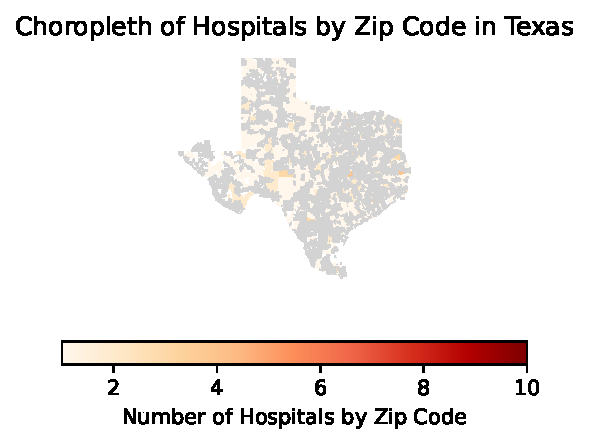
\includegraphics{Sujie- Abu Bakar_files/figure-pdf/cell-29-output-1.pdf}

\subsection{Calculate zip code's distance to the nearest hospital (20
pts)
(*)}\label{calculate-zip-codes-distance-to-the-nearest-hospital-20-pts}

\begin{enumerate}
\def\labelenumi{\arabic{enumi}.}
\tightlist
\item
\end{enumerate}

\begin{Shaded}
\begin{Highlighting}[]
\NormalTok{zips\_all\_centroids }\OperatorTok{=} \BuiltInTok{zip}\NormalTok{.copy().to\_crs(epsg}\OperatorTok{=}\DecValTok{32614}\NormalTok{)}
\NormalTok{zips\_all\_centroids[}\StringTok{"geometry"}\NormalTok{] }\OperatorTok{=}\NormalTok{ zips\_all\_centroids.centroid}
\NormalTok{dimensions }\OperatorTok{=}\NormalTok{ zips\_all\_centroids.shape}
\BuiltInTok{print}\NormalTok{(dimensions)}
\NormalTok{zips\_all\_centroids.head()}
\end{Highlighting}
\end{Shaded}

\begin{verbatim}
(33120, 6)
\end{verbatim}

\begin{longtable}[]{@{}lllllll@{}}
\toprule\noalign{}
& GEO\_ID & ZCTA5 & NAME & LSAD & CENSUSAREA & geometry \\
\midrule\noalign{}
\endhead
\bottomrule\noalign{}
\endlastfoot
0 & 8600000US01040 & 01040 & 01040 & ZCTA5 & 21.281 & POINT (2680901.614
5023480.354) \\
1 & 8600000US01050 & 01050 & 01050 & ZCTA5 & 38.329 & POINT (2659157.771
5025591.454) \\
2 & 8600000US01053 & 01053 & 01053 & ZCTA5 & 5.131 & POINT (2669825.294
5037254.622) \\
3 & 8600000US01056 & 01056 & 01056 & ZCTA5 & 27.205 & POINT (2696847.204
5026281.101) \\
4 & 8600000US01057 & 01057 & 01057 & ZCTA5 & 44.907 & POINT (2711728.101
5018798.677) \\
\end{longtable}

The dimension of this GeoDataFrame is (33120, 6). For each column,
\texttt{GEO\_ID} is the id, \texttt{ZCTA5} is the zip code,
\texttt{NAME} is the zip code as well, \texttt{CENSUSAREA} is the area,
\texttt{geometry} is the centroid of each zip code.

\begin{enumerate}
\def\labelenumi{\arabic{enumi}.}
\setcounter{enumi}{1}
\tightlist
\item
\end{enumerate}

\begin{Shaded}
\begin{Highlighting}[]
\NormalTok{texas\_prefixes }\OperatorTok{=}\NormalTok{ [}\StringTok{\textquotesingle{}75\textquotesingle{}}\NormalTok{, }\StringTok{\textquotesingle{}76\textquotesingle{}}\NormalTok{, }\StringTok{\textquotesingle{}77\textquotesingle{}}\NormalTok{, }\StringTok{\textquotesingle{}78\textquotesingle{}}\NormalTok{, }\StringTok{\textquotesingle{}79\textquotesingle{}}\NormalTok{, }\StringTok{\textquotesingle{}733\textquotesingle{}}\NormalTok{]}
\NormalTok{bordering\_states\_prefixes }\OperatorTok{=}\NormalTok{ texas\_prefixes }\OperatorTok{+}\NormalTok{ [}\StringTok{\textquotesingle{}73\textquotesingle{}}\NormalTok{, }\StringTok{\textquotesingle{}74\textquotesingle{}}\NormalTok{, }\StringTok{\textquotesingle{}70\textquotesingle{}}\NormalTok{, }\StringTok{\textquotesingle{}71\textquotesingle{}}\NormalTok{, }\StringTok{\textquotesingle{}87\textquotesingle{}}\NormalTok{, }\StringTok{\textquotesingle{}88\textquotesingle{}}\NormalTok{]}

\NormalTok{zips\_texas\_centroids }\OperatorTok{=}\NormalTok{ zips\_all\_centroids[zips\_all\_centroids[}\StringTok{\textquotesingle{}NAME\textquotesingle{}}\NormalTok{].}\BuiltInTok{str}\NormalTok{[:}\DecValTok{3}\NormalTok{].isin([}\StringTok{\textquotesingle{}733\textquotesingle{}}\NormalTok{]) }\OperatorTok{|}\NormalTok{ zips\_all\_centroids[}\StringTok{\textquotesingle{}NAME\textquotesingle{}}\NormalTok{].}\BuiltInTok{str}\NormalTok{[:}\DecValTok{2}\NormalTok{].isin([}\StringTok{\textquotesingle{}75\textquotesingle{}}\NormalTok{, }\StringTok{\textquotesingle{}76\textquotesingle{}}\NormalTok{, }\StringTok{\textquotesingle{}77\textquotesingle{}}\NormalTok{, }\StringTok{\textquotesingle{}78\textquotesingle{}}\NormalTok{, }\StringTok{\textquotesingle{}79\textquotesingle{}}\NormalTok{])].copy()}

\NormalTok{zips\_texas\_centroids }\OperatorTok{=}\NormalTok{ zips\_texas\_centroids.to\_crs(epsg}\OperatorTok{=}\DecValTok{32614}\NormalTok{)}

\NormalTok{zips\_texas\_borderstates\_centroids }\OperatorTok{=}\NormalTok{ zips\_all\_centroids[zips\_all\_centroids[}\StringTok{\textquotesingle{}NAME\textquotesingle{}}\NormalTok{].}\BuiltInTok{str}\NormalTok{[:}\DecValTok{2}\NormalTok{].isin(bordering\_states\_prefixes)].copy()}

\NormalTok{zips\_texas\_borderstates\_centroids }\OperatorTok{=}\NormalTok{ zips\_texas\_borderstates\_centroids.to\_crs(epsg}\OperatorTok{=}\DecValTok{32614}\NormalTok{)}

\NormalTok{texas\_zip\_count }\OperatorTok{=}\NormalTok{ zips\_texas\_centroids[}\StringTok{\textquotesingle{}NAME\textquotesingle{}}\NormalTok{].nunique()}
\NormalTok{texas\_borderstates\_zip\_count }\OperatorTok{=}\NormalTok{ zips\_texas\_borderstates\_centroids[}\StringTok{\textquotesingle{}NAME\textquotesingle{}}\NormalTok{].nunique()}

\BuiltInTok{print}\NormalTok{(}\SpecialStringTok{f"There are }\SpecialCharTok{\{}\NormalTok{texas\_zip\_count}\SpecialCharTok{\}}\SpecialStringTok{ unique zip codes zips\_texas\_centroids subsets."}\NormalTok{)}
\BuiltInTok{print}\NormalTok{(}\SpecialStringTok{f"There are }\SpecialCharTok{\{}\NormalTok{texas\_borderstates\_zip\_count}\SpecialCharTok{\}}\SpecialStringTok{ unique zip codes zips\_texas\_borderstates\_centroids subsets."}\NormalTok{)}
\end{Highlighting}
\end{Shaded}

\begin{verbatim}
There are 1935 unique zip codes zips_texas_centroids subsets.
There are 3596 unique zip codes zips_texas_borderstates_centroids subsets.
\end{verbatim}

\begin{Shaded}
\begin{Highlighting}[]
\NormalTok{zips\_texas\_centroids.head()}
\end{Highlighting}
\end{Shaded}

\begin{longtable}[]{@{}lllllll@{}}
\toprule\noalign{}
& GEO\_ID & ZCTA5 & NAME & LSAD & CENSUSAREA & geometry \\
\midrule\noalign{}
\endhead
\bottomrule\noalign{}
\endlastfoot
9207 & 8600000US78624 & 78624 & 78624 & ZCTA5 & 708.041 & POINT
(511823.895 3349990.765) \\
9208 & 8600000US78626 & 78626 & 78626 & ZCTA5 & 93.046 & POINT
(634378.798 3393352.86) \\
9209 & 8600000US78628 & 78628 & 78628 & ZCTA5 & 73.382 & POINT
(619673.552 3390490.031) \\
9210 & 8600000US78631 & 78631 & 78631 & ZCTA5 & 325.074 & POINT
(470662.193 3356245.449) \\
9211 & 8600000US78632 & 78632 & 78632 & ZCTA5 & 96.278 & POINT
(647977.423 3286112.808) \\
\end{longtable}

\begin{enumerate}
\def\labelenumi{\arabic{enumi}.}
\setcounter{enumi}{2}
\tightlist
\item
\end{enumerate}

\begin{Shaded}
\begin{Highlighting}[]
\NormalTok{zips\_texas\_borderstates\_centroids }\OperatorTok{=}\NormalTok{ zips\_texas\_borderstates\_centroids.to\_crs(epsg}\OperatorTok{=}\DecValTok{32614}\NormalTok{)}
\NormalTok{count\_zip2016 }\OperatorTok{=}\NormalTok{ pd.DataFrame(count\_zip2016)}
\NormalTok{count\_zip2016[}\StringTok{\textquotesingle{}ZIP\_CD\textquotesingle{}}\NormalTok{] }\OperatorTok{=}\NormalTok{ count\_zip2016[}\StringTok{\textquotesingle{}ZIP\_CD\textquotesingle{}}\NormalTok{].fillna(}\DecValTok{0}\NormalTok{)}
\NormalTok{count\_zip2016.loc[:, }\StringTok{\textquotesingle{}ZIP\_CD\textquotesingle{}}\NormalTok{] }\OperatorTok{=}\NormalTok{ count\_zip2016[}\StringTok{\textquotesingle{}ZIP\_CD\textquotesingle{}}\NormalTok{].astype(}\BuiltInTok{int}\NormalTok{).astype(}\BuiltInTok{str}\NormalTok{).}\BuiltInTok{str}\NormalTok{.zfill(}\DecValTok{5}\NormalTok{)}
\NormalTok{zips\_withhospital\_centroids }\OperatorTok{=}\NormalTok{ zips\_texas\_borderstates\_centroids.merge(}
\NormalTok{    count\_zip2016,}
\NormalTok{    left\_on}\OperatorTok{=}\StringTok{\textquotesingle{}NAME\textquotesingle{}}\NormalTok{,}
\NormalTok{    right\_on}\OperatorTok{=}\StringTok{\textquotesingle{}ZIP\_CD\textquotesingle{}}\NormalTok{,}
\NormalTok{    how}\OperatorTok{=}\StringTok{\textquotesingle{}inner\textquotesingle{}}
\NormalTok{)}
\end{Highlighting}
\end{Shaded}

\begin{verbatim}
/var/folders/zc/d18v235x3mn0wtlnmmwm3_4c0000gn/T/ipykernel_13910/2177933344.py:4: FutureWarning: Setting an item of incompatible dtype is deprecated and will raise in a future error of pandas. Value '['00603' '00613' '00614' ... '99835' '99901' '99929']' has dtype incompatible with float64, please explicitly cast to a compatible dtype first.
  count_zip2016.loc[:, 'ZIP_CD'] = count_zip2016['ZIP_CD'].astype(int).astype(str).str.zfill(5)
\end{verbatim}

I choose inner merge, with \texttt{NAME} variable for
\texttt{zips\_texas\_borderstates\_centroids} and \texttt{ZIP\_CD}
variable for \texttt{count\_zip2016}. Both \texttt{NAME} and
\texttt{ZIP\_CD} represent the zip code.

\begin{enumerate}
\def\labelenumi{\arabic{enumi}.}
\setcounter{enumi}{3}
\tightlist
\item
  \begin{enumerate}
  \def\labelenumii{\alph{enumii}.}
  \tightlist
  \item
  \end{enumerate}
\end{enumerate}

\begin{Shaded}
\begin{Highlighting}[]
\NormalTok{zips\_texas\_centroids\_10 }\OperatorTok{=}\NormalTok{ zips\_texas\_centroids.head(}\DecValTok{10}\NormalTok{)}
\NormalTok{zips\_texas\_centroids\_10 }\OperatorTok{=}\NormalTok{ zips\_texas\_centroids\_10.to\_crs(epsg}\OperatorTok{=}\DecValTok{4326}\NormalTok{)}
\NormalTok{zips\_texas\_centroids\_10}
\NormalTok{zips\_withhospital\_centroids }\OperatorTok{=}\NormalTok{ zips\_withhospital\_centroids.to\_crs(epsg}\OperatorTok{=}\DecValTok{4326}\NormalTok{)}
\end{Highlighting}
\end{Shaded}

\begin{Shaded}
\begin{Highlighting}[]
\CommentTok{\# Convert both GeoDataFrames to a suitable projected CRS (NAD83 / Texas Central, EPSG:2272)}
\NormalTok{zips\_texas\_centroids\_10 }\OperatorTok{=}\NormalTok{ zips\_texas\_centroids\_10.to\_crs(epsg}\OperatorTok{=}\DecValTok{2272}\NormalTok{)  }
\NormalTok{zips\_withhospital\_centroids }\OperatorTok{=}\NormalTok{ zips\_withhospital\_centroids.to\_crs(epsg}\OperatorTok{=}\DecValTok{2272}\NormalTok{)}

\ImportTok{import}\NormalTok{ time}
\NormalTok{start\_time }\OperatorTok{=}\NormalTok{ time.time()}

\NormalTok{nearest\_distances }\OperatorTok{=}\NormalTok{ []}

\CommentTok{\# Calculate the nearest distance for each zip code}
\ControlFlowTok{for}\NormalTok{ \_, zip\_row }\KeywordTok{in}\NormalTok{ zips\_texas\_centroids\_10.iterrows():}
    \CommentTok{\# Calculate distance to all hospitals}
\NormalTok{    distances }\OperatorTok{=}\NormalTok{ zips\_withhospital\_centroids.geometry.distance(zip\_row.geometry)}
    \CommentTok{\# Get the minimum distance}
\NormalTok{    nearest\_distance }\OperatorTok{=}\NormalTok{ distances.}\BuiltInTok{min}\NormalTok{()}
\NormalTok{    nearest\_distances.append(nearest\_distance)}

\CommentTok{\# Add the nearest distances to the GeoDataFrame}
\NormalTok{zips\_texas\_centroids\_10[}\StringTok{\textquotesingle{}nearest\_hospital\_distance\textquotesingle{}}\NormalTok{] }\OperatorTok{=}\NormalTok{ nearest\_distances}

\NormalTok{end\_time }\OperatorTok{=}\NormalTok{ time.time()}
\BuiltInTok{print}\NormalTok{(}\SpecialStringTok{f"Execution time: }\SpecialCharTok{\{}\NormalTok{end\_time }\OperatorTok{{-}}\NormalTok{ start\_time}\SpecialCharTok{:.2f\}}\SpecialStringTok{ seconds"}\NormalTok{)}
\end{Highlighting}
\end{Shaded}

\begin{verbatim}
Execution time: 0.02 seconds
\end{verbatim}

For 10 records, it takes 0.02 seconds. For there are 1935 records, I
think the total calculation time is 0.02 * 193 = 4 seconds.

\begin{verbatim}
b.
\end{verbatim}

\begin{Shaded}
\begin{Highlighting}[]
\NormalTok{start\_time }\OperatorTok{=}\NormalTok{ time.time()}

\NormalTok{nearest\_distances }\OperatorTok{=}\NormalTok{ []}

\CommentTok{\# Calculate the nearest distance for each zip code}
\ControlFlowTok{for}\NormalTok{ \_, zip\_row }\KeywordTok{in}\NormalTok{ zips\_texas\_centroids.iterrows():}
    \CommentTok{\# Calculate distance to all hospitals}
\NormalTok{    distances }\OperatorTok{=}\NormalTok{ zips\_withhospital\_centroids.geometry.distance(zip\_row.geometry)}
    \CommentTok{\# Get the minimum distance}
\NormalTok{    nearest\_distance }\OperatorTok{=}\NormalTok{ distances.}\BuiltInTok{min}\NormalTok{()}
\NormalTok{    nearest\_distances.append(nearest\_distance)}

\CommentTok{\# Add the nearest distances to the GeoDataFrame}
\NormalTok{zips\_texas\_centroids[}\StringTok{\textquotesingle{}nearest\_hospital\_distance\textquotesingle{}}\NormalTok{] }\OperatorTok{=}\NormalTok{ nearest\_distances}

\NormalTok{end\_time }\OperatorTok{=}\NormalTok{ time.time()}
\BuiltInTok{print}\NormalTok{(}\SpecialStringTok{f"Execution time: }\SpecialCharTok{\{}\NormalTok{end\_time }\OperatorTok{{-}}\NormalTok{ start\_time}\SpecialCharTok{:.2f\}}\SpecialStringTok{ seconds"}\NormalTok{)}
\end{Highlighting}
\end{Shaded}

\begin{verbatim}
Execution time: 2.06 seconds
\end{verbatim}

The difference is close.

\begin{enumerate}
\def\labelenumi{\alph{enumi}.}
\setcounter{enumi}{2}
\tightlist
\item
\end{enumerate}

\begin{Shaded}
\begin{Highlighting}[]
\ControlFlowTok{with} \BuiltInTok{open}\NormalTok{(filepath2, }\StringTok{\textquotesingle{}r\textquotesingle{}}\NormalTok{) }\ImportTok{as} \BuiltInTok{file}\NormalTok{:}
\NormalTok{    prj\_content }\OperatorTok{=} \BuiltInTok{file}\NormalTok{.read()}
\BuiltInTok{print}\NormalTok{(prj\_content)}
\end{Highlighting}
\end{Shaded}

\begin{verbatim}
GEOGCS["GCS_North_American_1983",DATUM["D_North_American_1983",SPHEROID["GRS_1980",6378137,298.257222101]],PRIMEM["Greenwich",0],UNIT["Degree",0.017453292519943295]]
\end{verbatim}

\begin{enumerate}
\def\labelenumi{\arabic{enumi}.}
\setcounter{enumi}{4}
\item
  \begin{enumerate}
  \def\labelenumii{\alph{enumii}.}
  \item
    It is in feet now becasue I reprojected it to EPSG:2272
  \item
  \end{enumerate}
\end{enumerate}

\begin{Shaded}
\begin{Highlighting}[]
\NormalTok{zips\_texas\_centroids }\OperatorTok{=}\NormalTok{ zips\_texas\_centroids.to\_crs(epsg}\OperatorTok{=}\DecValTok{2272}\NormalTok{)}
\NormalTok{zips\_withhospital\_centroids }\OperatorTok{=}\NormalTok{ zips\_withhospital\_centroids.to\_crs(epsg}\OperatorTok{=}\DecValTok{2272}\NormalTok{)}

\CommentTok{\# Initialize a list to store nearest hospital distances for each ZIP centroid}
\NormalTok{nearest\_distances }\OperatorTok{=}\NormalTok{ []}

\CommentTok{\# Calculate the minimum distance for each ZIP centroid in Texas to the nearest hospital centroid}
\ControlFlowTok{for}\NormalTok{ \_, zip\_row }\KeywordTok{in}\NormalTok{ zips\_texas\_centroids.iterrows():}
\NormalTok{    distances }\OperatorTok{=}\NormalTok{ zips\_withhospital\_centroids.geometry.distance(zip\_row.geometry)}
\NormalTok{    nearest\_distance }\OperatorTok{=}\NormalTok{ distances.}\BuiltInTok{min}\NormalTok{()  }\CommentTok{\# Minimum distance to the nearest hospital}
\NormalTok{    nearest\_distances.append(nearest\_distance)}

\CommentTok{\# Add the calculated distances (in feet) to the GeoDataFrame and convert to miles}
\NormalTok{zips\_texas\_centroids[}\StringTok{\textquotesingle{}nearest\_hospital\_distance\_feet\textquotesingle{}}\NormalTok{] }\OperatorTok{=}\NormalTok{ nearest\_distances}
\NormalTok{zips\_texas\_centroids[}\StringTok{\textquotesingle{}nearest\_hospital\_distance\_miles\textquotesingle{}}\NormalTok{] }\OperatorTok{=}\NormalTok{ zips\_texas\_centroids[}\StringTok{\textquotesingle{}nearest\_hospital\_distance\_feet\textquotesingle{}}\NormalTok{] }\OperatorTok{/} \DecValTok{5280}

\CommentTok{\# Calculate and display the average distance to the nearest hospital (in miles)}
\NormalTok{average\_distance\_miles }\OperatorTok{=}\NormalTok{ zips\_texas\_centroids[}\StringTok{\textquotesingle{}nearest\_hospital\_distance\_miles\textquotesingle{}}\NormalTok{].mean()}
\BuiltInTok{print}\NormalTok{(}\SpecialStringTok{f"Average distance to the nearest hospital in miles: }\SpecialCharTok{\{}\NormalTok{average\_distance\_miles}\SpecialCharTok{:.2f\}}\SpecialStringTok{"}\NormalTok{)}
\end{Highlighting}
\end{Shaded}

\begin{verbatim}
Average distance to the nearest hospital in miles: 8.29
\end{verbatim}

\begin{verbatim}
c.
\end{verbatim}

\begin{Shaded}
\begin{Highlighting}[]
\CommentTok{\# Plot the map}
\NormalTok{fig, ax }\OperatorTok{=}\NormalTok{ plt.subplots(}\DecValTok{1}\NormalTok{, }\DecValTok{1}\NormalTok{, figsize}\OperatorTok{=}\NormalTok{(}\DecValTok{4}\NormalTok{, }\DecValTok{3}\NormalTok{))}
\NormalTok{zips\_texas\_centroids.plot(column}\OperatorTok{=}\StringTok{\textquotesingle{}nearest\_hospital\_distance\_miles\textquotesingle{}}\NormalTok{, }
\NormalTok{                          ax}\OperatorTok{=}\NormalTok{ax, }
\NormalTok{                          legend}\OperatorTok{=}\VariableTok{True}\NormalTok{, }
\NormalTok{                          legend\_kwds}\OperatorTok{=}\NormalTok{\{}\StringTok{\textquotesingle{}label\textquotesingle{}}\NormalTok{: }\StringTok{"Distance to Nearest Hospital (miles)"}\NormalTok{, }\StringTok{\textquotesingle{}orientation\textquotesingle{}}\NormalTok{: }\StringTok{"horizontal"}\NormalTok{\},}
\NormalTok{                          cmap}\OperatorTok{=}\StringTok{\textquotesingle{}OrRd\textquotesingle{}}\NormalTok{,  }\CommentTok{\# Choose an appropriate color map}
\NormalTok{                          missing\_kwds}\OperatorTok{=}\NormalTok{\{}\StringTok{\textquotesingle{}color\textquotesingle{}}\NormalTok{: }\StringTok{\textquotesingle{}lightgrey\textquotesingle{}}\NormalTok{\})  }\CommentTok{\# Color for missing values}

\CommentTok{\# Customize the plot}
\NormalTok{ax.set\_title(}\StringTok{\textquotesingle{}Average Distance to Nearest Hospital by ZIP Code\textquotesingle{}}\NormalTok{)}
\NormalTok{ax.set\_axis\_off()  }\CommentTok{\# Hide the axis for a cleaner map}

\NormalTok{plt.show()}
\end{Highlighting}
\end{Shaded}

\includegraphics{Sujie- Abu Bakar_files/figure-pdf/cell-39-output-1.pdf}

\subsection{Effects of closures on access in Texas (15
pts)}\label{effects-of-closures-on-access-in-texas-15-pts}

\begin{enumerate}
\def\labelenumi{\arabic{enumi}.}
\tightlist
\item
\end{enumerate}

\begin{Shaded}
\begin{Highlighting}[]
\NormalTok{corrected\_closures}

\NormalTok{corrected\_closures[}\StringTok{\textquotesingle{}ZIP\_CD\textquotesingle{}}\NormalTok{] }\OperatorTok{=}\NormalTok{ corrected\_closures[}\StringTok{\textquotesingle{}ZIP\_CD\textquotesingle{}}\NormalTok{].astype(}\BuiltInTok{str}\NormalTok{)}

\CommentTok{\# Filter the corrected closures dataset to include only ZIP codes in Texas and closures from 2016 to 2019}
\NormalTok{texas\_closures }\OperatorTok{=}\NormalTok{ corrected\_closures[}
\NormalTok{    (corrected\_closures[}\StringTok{\textquotesingle{}ZIP\_CD\textquotesingle{}}\NormalTok{].}\BuiltInTok{str}\NormalTok{.startswith(}\StringTok{\textquotesingle{}75\textquotesingle{}}\NormalTok{) }\OperatorTok{|}  \CommentTok{\# Common Texas ZIP code prefixes}
\NormalTok{     corrected\_closures[}\StringTok{\textquotesingle{}ZIP\_CD\textquotesingle{}}\NormalTok{].}\BuiltInTok{str}\NormalTok{.startswith(}\StringTok{\textquotesingle{}76\textquotesingle{}}\NormalTok{) }\OperatorTok{|}
\NormalTok{     corrected\_closures[}\StringTok{\textquotesingle{}ZIP\_CD\textquotesingle{}}\NormalTok{].}\BuiltInTok{str}\NormalTok{.startswith(}\StringTok{\textquotesingle{}77\textquotesingle{}}\NormalTok{) }\OperatorTok{|}
\NormalTok{     corrected\_closures[}\StringTok{\textquotesingle{}ZIP\_CD\textquotesingle{}}\NormalTok{].}\BuiltInTok{str}\NormalTok{.startswith(}\StringTok{\textquotesingle{}78\textquotesingle{}}\NormalTok{) }\OperatorTok{|}
\NormalTok{     corrected\_closures[}\StringTok{\textquotesingle{}ZIP\_CD\textquotesingle{}}\NormalTok{].}\BuiltInTok{str}\NormalTok{.startswith(}\StringTok{\textquotesingle{}79\textquotesingle{}}\NormalTok{) }\OperatorTok{|}
\NormalTok{     corrected\_closures[}\StringTok{\textquotesingle{}ZIP\_CD\textquotesingle{}}\NormalTok{].}\BuiltInTok{str}\NormalTok{.startswith(}\StringTok{\textquotesingle{}733\textquotesingle{}}\NormalTok{))}
\NormalTok{]}

\CommentTok{\# Count the number of closures by ZIP code}
\NormalTok{closures\_by\_zip }\OperatorTok{=}\NormalTok{ texas\_closures.groupby(}\StringTok{\textquotesingle{}ZIP\_CD\textquotesingle{}}\NormalTok{).size().reset\_index(name}\OperatorTok{=}\StringTok{\textquotesingle{}closure\_count\textquotesingle{}}\NormalTok{)}

\ImportTok{import}\NormalTok{ numpy }\ImportTok{as}\NormalTok{ np}
\CommentTok{\# Display the table of the number of closures by ZIP code}
\BuiltInTok{print}\NormalTok{(}\StringTok{"Table of the number of closures by ZIP code in Texas (2016{-}2019):"}\NormalTok{)}
\NormalTok{closures\_by\_zip[}\StringTok{\textquotesingle{}ZIP\_CD\textquotesingle{}}\NormalTok{] }\OperatorTok{=}\NormalTok{ closures\_by\_zip[}\StringTok{\textquotesingle{}ZIP\_CD\textquotesingle{}}\NormalTok{].astype(}\BuiltInTok{float}\NormalTok{).astype(}\BuiltInTok{int}\NormalTok{).astype(}\BuiltInTok{str}\NormalTok{).}\BuiltInTok{str}\NormalTok{.zfill(}\DecValTok{5}\NormalTok{)}
\NormalTok{closures\_by\_zip}
\end{Highlighting}
\end{Shaded}

\begin{verbatim}
Table of the number of closures by ZIP code in Texas (2016-2019):
\end{verbatim}

\begin{longtable}[]{@{}lll@{}}
\toprule\noalign{}
& ZIP\_CD & closure\_count \\
\midrule\noalign{}
\endhead
\bottomrule\noalign{}
\endlastfoot
0 & 75662 & 1 \\
1 & 75835 & 1 \\
2 & 75862 & 1 \\
3 & 76502 & 1 \\
4 & 77035 & 1 \\
5 & 78017 & 1 \\
6 & 78061 & 1 \\
7 & 78734 & 1 \\
8 & 78834 & 1 \\
9 & 79735 & 1 \\
\end{longtable}

\begin{enumerate}
\def\labelenumi{\arabic{enumi}.}
\setcounter{enumi}{1}
\tightlist
\item
\end{enumerate}

\begin{Shaded}
\begin{Highlighting}[]
\CommentTok{\# Ensure ZIP\_CD in closures\_by\_zip and texas\_zip\_shapes are the same format}
\NormalTok{zip\_tx[}\StringTok{\textquotesingle{}ZIP\_CD\textquotesingle{}}\NormalTok{] }\OperatorTok{=}\NormalTok{ zip\_tx[}\StringTok{\textquotesingle{}ZIP\_CD\textquotesingle{}}\NormalTok{].astype(}\BuiltInTok{str}\NormalTok{).}\BuiltInTok{str}\NormalTok{.zfill(}\DecValTok{5}\NormalTok{)}

\CommentTok{\# Merge the geographic data with the closure data}
\NormalTok{texas\_closures\_geo }\OperatorTok{=}\NormalTok{ zip\_tx.merge(closures\_by\_zip, on}\OperatorTok{=}\StringTok{\textquotesingle{}ZIP\_CD\textquotesingle{}}\NormalTok{, how}\OperatorTok{=}\StringTok{\textquotesingle{}left\textquotesingle{}}\NormalTok{).fillna(}\DecValTok{0}\NormalTok{)}

\CommentTok{\# Plot the choropleth map}
\NormalTok{fig, ax }\OperatorTok{=}\NormalTok{ plt.subplots(}\DecValTok{1}\NormalTok{, }\DecValTok{1}\NormalTok{, figsize}\OperatorTok{=}\NormalTok{(}\DecValTok{4}\NormalTok{, }\DecValTok{3}\NormalTok{))}
\NormalTok{texas\_closures\_geo.plot(column}\OperatorTok{=}\StringTok{\textquotesingle{}closure\_count\textquotesingle{}}\NormalTok{, ax}\OperatorTok{=}\NormalTok{ax, legend}\OperatorTok{=}\VariableTok{True}\NormalTok{,}
\NormalTok{                        legend\_kwds}\OperatorTok{=}\NormalTok{\{}\StringTok{\textquotesingle{}label\textquotesingle{}}\NormalTok{: }\StringTok{"Number of Closures (2016{-}2019)"}\NormalTok{, }\StringTok{\textquotesingle{}orientation\textquotesingle{}}\NormalTok{: }\StringTok{"horizontal"}\NormalTok{\},}
\NormalTok{                        cmap}\OperatorTok{=}\StringTok{\textquotesingle{}OrRd\textquotesingle{}}\NormalTok{,  }\CommentTok{\# color map for the intensity of closures}
\NormalTok{                        missing\_kwds}\OperatorTok{=}\NormalTok{\{}\StringTok{\textquotesingle{}color\textquotesingle{}}\NormalTok{: }\StringTok{\textquotesingle{}lightgrey\textquotesingle{}}\NormalTok{\})  }\CommentTok{\# Color for areas with no data}

\CommentTok{\# Customize the plot}
\NormalTok{ax.set\_title(}\StringTok{\textquotesingle{}Hospital Closures in Texas by ZIP Code (2016{-}2019)\textquotesingle{}}\NormalTok{)}
\NormalTok{ax.set\_axis\_off()  }\CommentTok{\# Hide axis for a cleaner map}

\NormalTok{plt.show()}

\CommentTok{\# Count the number of directly affected ZIP codes in Texas}
\NormalTok{num\_affected\_zip\_codes }\OperatorTok{=}\NormalTok{ closures\_by\_zip[}\StringTok{\textquotesingle{}ZIP\_CD\textquotesingle{}}\NormalTok{].nunique()}
\BuiltInTok{print}\NormalTok{(}\SpecialStringTok{f"Number of directly affected ZIP codes in Texas: }\SpecialCharTok{\{}\NormalTok{num\_affected\_zip\_codes}\SpecialCharTok{\}}\SpecialStringTok{"}\NormalTok{)}
\end{Highlighting}
\end{Shaded}

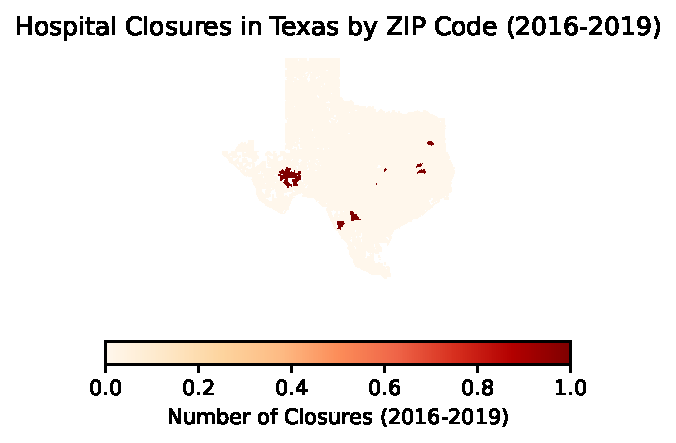
\includegraphics{Sujie- Abu Bakar_files/figure-pdf/cell-41-output-1.pdf}

\begin{verbatim}
Number of directly affected ZIP codes in Texas: 10
\end{verbatim}

\begin{enumerate}
\def\labelenumi{\arabic{enumi}.}
\setcounter{enumi}{2}
\tightlist
\item
\end{enumerate}

\begin{Shaded}
\begin{Highlighting}[]
\CommentTok{\# Filter the directly affected ZIP codes from \textasciigrave{}closures\_by\_zip\textasciigrave{}}
\NormalTok{affected\_zips }\OperatorTok{=}\NormalTok{ closures\_by\_zip[closures\_by\_zip[}\StringTok{\textquotesingle{}closure\_count\textquotesingle{}}\NormalTok{] }\OperatorTok{\textgreater{}} \DecValTok{0}\NormalTok{][}\StringTok{\textquotesingle{}ZIP\_CD\textquotesingle{}}\NormalTok{].unique()}

\CommentTok{\# Convert \textasciigrave{}closures\_by\_zip\textasciigrave{} to a GeoDataFrame with directly affected ZIP codes only}
\NormalTok{directly\_affected\_geo }\OperatorTok{=}\NormalTok{ zip\_tx[zip\_tx[}\StringTok{\textquotesingle{}ZIP\_CD\textquotesingle{}}\NormalTok{].isin(affected\_zips)]}

\CommentTok{\# Convert the GeoDataFrame to a projected coordinate system (e.g., EPSG:2272) for accurate distance{-}based operations}
\NormalTok{directly\_affected\_geo }\OperatorTok{=}\NormalTok{ directly\_affected\_geo.to\_crs(epsg}\OperatorTok{=}\DecValTok{2272}\NormalTok{)}
\NormalTok{texas\_zip\_shapes }\OperatorTok{=}\NormalTok{ zip\_tx.to\_crs(epsg}\OperatorTok{=}\DecValTok{2272}\NormalTok{)}

\CommentTok{\# Create a 10{-}mile buffer around each directly affected ZIP code}
\CommentTok{\# 1 mile is approximately 1609.34 meters}
\NormalTok{buffer\_distance }\OperatorTok{=} \DecValTok{10} \OperatorTok{*} \FloatTok{1609.34}  \CommentTok{\# 10 miles in meters}
\NormalTok{directly\_affected\_geo[}\StringTok{\textquotesingle{}geometry\textquotesingle{}}\NormalTok{] }\OperatorTok{=}\NormalTok{ directly\_affected\_geo.}\BuiltInTok{buffer}\NormalTok{(buffer\_distance)}

\CommentTok{\# Perform a spatial join to find ZIP codes within the 10{-}mile buffer of directly affected ZIP codes}
\NormalTok{indirectly\_affected\_geo }\OperatorTok{=}\NormalTok{ gpd.sjoin(texas\_zip\_shapes, directly\_affected\_geo, how}\OperatorTok{=}\StringTok{\textquotesingle{}inner\textquotesingle{}}\NormalTok{, predicate}\OperatorTok{=}\StringTok{\textquotesingle{}intersects\textquotesingle{}}\NormalTok{)}

\CommentTok{\# Count unique indirectly affected ZIP codes}
\NormalTok{indirectly\_affected\_zip\_count }\OperatorTok{=}\NormalTok{ indirectly\_affected\_geo[}\StringTok{\textquotesingle{}ZIP\_CD\_left\textquotesingle{}}\NormalTok{].nunique() }\OperatorTok{{-}} \BuiltInTok{len}\NormalTok{(affected\_zips)}

\CommentTok{\# Display results}
\BuiltInTok{print}\NormalTok{(}\SpecialStringTok{f"Number of indirectly affected ZIP codes in Texas: }\SpecialCharTok{\{}\NormalTok{indirectly\_affected\_zip\_count}\SpecialCharTok{\}}\SpecialStringTok{"}\NormalTok{)}
\end{Highlighting}
\end{Shaded}

\begin{verbatim}
Number of indirectly affected ZIP codes in Texas: 95
\end{verbatim}

\begin{enumerate}
\def\labelenumi{\arabic{enumi}.}
\setcounter{enumi}{3}
\tightlist
\item
\end{enumerate}

\begin{Shaded}
\begin{Highlighting}[]
\CommentTok{\# Step 1: Prepare the Texas ZIP shapes and classify each ZIP code}

\CommentTok{\# Step 1.1: Create a list of directly affected ZIP codes}
\NormalTok{directly\_affected\_zips }\OperatorTok{=}\NormalTok{ closures\_by\_zip[closures\_by\_zip[}\StringTok{\textquotesingle{}closure\_count\textquotesingle{}}\NormalTok{] }\OperatorTok{\textgreater{}} \DecValTok{0}\NormalTok{][}\StringTok{\textquotesingle{}ZIP\_CD\textquotesingle{}}\NormalTok{].unique()}

\CommentTok{\# Step 1.2: Create the directly affected GeoDataFrame}
\NormalTok{directly\_affected\_geo }\OperatorTok{=}\NormalTok{ zip\_tx[zip\_tx[}\StringTok{\textquotesingle{}ZIP\_CD\textquotesingle{}}\NormalTok{].isin(directly\_affected\_zips)]}

\CommentTok{\# Convert to a projected CRS for distance calculation (e.g., EPSG:2272)}
\NormalTok{directly\_affected\_geo }\OperatorTok{=}\NormalTok{ directly\_affected\_geo.to\_crs(epsg}\OperatorTok{=}\DecValTok{2272}\NormalTok{)}
\NormalTok{texas\_zip\_shapes }\OperatorTok{=}\NormalTok{ texas\_zip\_shapes.to\_crs(epsg}\OperatorTok{=}\DecValTok{2272}\NormalTok{)}

\CommentTok{\# Step 1.3: Create a 10{-}mile buffer around each directly affected ZIP code}
\NormalTok{buffer\_distance }\OperatorTok{=} \DecValTok{10} \OperatorTok{*} \FloatTok{1609.34}  \CommentTok{\# 10 miles in meters}
\NormalTok{directly\_affected\_geo[}\StringTok{\textquotesingle{}geometry\textquotesingle{}}\NormalTok{] }\OperatorTok{=}\NormalTok{ directly\_affected\_geo.}\BuiltInTok{buffer}\NormalTok{(buffer\_distance)}

\CommentTok{\# Step 1.4: Perform a spatial join to identify indirectly affected ZIP codes}
\NormalTok{indirectly\_affected\_geo }\OperatorTok{=}\NormalTok{ gpd.sjoin(texas\_zip\_shapes, directly\_affected\_geo, how}\OperatorTok{=}\StringTok{\textquotesingle{}inner\textquotesingle{}}\NormalTok{, predicate}\OperatorTok{=}\StringTok{\textquotesingle{}intersects\textquotesingle{}}\NormalTok{)}
\NormalTok{indirectly\_affected\_zips }\OperatorTok{=}\NormalTok{ indirectly\_affected\_geo[}\StringTok{\textquotesingle{}ZIP\_CD\_left\textquotesingle{}}\NormalTok{].unique()}

\CommentTok{\# Step 1.5: Classify ZIP codes}
\CommentTok{\# Initialize a column to classify each ZIP code}
\NormalTok{texas\_zip\_shapes[}\StringTok{\textquotesingle{}closure\_category\textquotesingle{}}\NormalTok{] }\OperatorTok{=} \StringTok{\textquotesingle{}Not Affected\textquotesingle{}}

\CommentTok{\# Mark directly affected ZIP codes}
\NormalTok{texas\_zip\_shapes.loc[texas\_zip\_shapes[}\StringTok{\textquotesingle{}ZIP\_CD\textquotesingle{}}\NormalTok{].isin(directly\_affected\_zips), }\StringTok{\textquotesingle{}closure\_category\textquotesingle{}}\NormalTok{] }\OperatorTok{=} \StringTok{\textquotesingle{}Directly Affected\textquotesingle{}}

\CommentTok{\# Mark indirectly affected ZIP codes (exclude directly affected ones)}
\NormalTok{texas\_zip\_shapes.loc[}
\NormalTok{    (texas\_zip\_shapes[}\StringTok{\textquotesingle{}ZIP\_CD\textquotesingle{}}\NormalTok{].isin(indirectly\_affected\_zips)) }\OperatorTok{\&} 
\NormalTok{    (}\OperatorTok{\textasciitilde{}}\NormalTok{texas\_zip\_shapes[}\StringTok{\textquotesingle{}ZIP\_CD\textquotesingle{}}\NormalTok{].isin(directly\_affected\_zips)), }
    \StringTok{\textquotesingle{}closure\_category\textquotesingle{}}
\NormalTok{] }\OperatorTok{=} \StringTok{\textquotesingle{}Indirectly Affected\textquotesingle{}}

\CommentTok{\# Step 2: Plot the choropleth map}

\CommentTok{\# Define a color map for the categories}
\NormalTok{category\_colors }\OperatorTok{=}\NormalTok{ \{}
    \StringTok{\textquotesingle{}Not Affected\textquotesingle{}}\NormalTok{: }\StringTok{\textquotesingle{}lightgrey\textquotesingle{}}\NormalTok{,}
    \StringTok{\textquotesingle{}Directly Affected\textquotesingle{}}\NormalTok{: }\StringTok{\textquotesingle{}red\textquotesingle{}}\NormalTok{,}
    \StringTok{\textquotesingle{}Indirectly Affected\textquotesingle{}}\NormalTok{: }\StringTok{\textquotesingle{}orange\textquotesingle{}}
\NormalTok{\}}

\NormalTok{fig, ax }\OperatorTok{=}\NormalTok{ plt.subplots(}\DecValTok{1}\NormalTok{, }\DecValTok{1}\NormalTok{, figsize}\OperatorTok{=}\NormalTok{(}\DecValTok{4}\NormalTok{, }\DecValTok{3}\NormalTok{))}
\NormalTok{texas\_zip\_shapes.plot(column}\OperatorTok{=}\StringTok{\textquotesingle{}closure\_category\textquotesingle{}}\NormalTok{, }
\NormalTok{                      ax}\OperatorTok{=}\NormalTok{ax, }
\NormalTok{                      legend}\OperatorTok{=}\VariableTok{True}\NormalTok{,}
\NormalTok{                      categorical}\OperatorTok{=}\VariableTok{True}\NormalTok{,}
\NormalTok{                      cmap}\OperatorTok{=}\StringTok{\textquotesingle{}Set1\textquotesingle{}}\NormalTok{,}
\NormalTok{                      legend\_kwds}\OperatorTok{=}\NormalTok{\{}\StringTok{\textquotesingle{}title\textquotesingle{}}\NormalTok{: }\StringTok{"Closure Impact Category"}\NormalTok{\})}

\CommentTok{\# Customize the plot}
\NormalTok{ax.set\_title(}\StringTok{\textquotesingle{}Texas ZIP Codes by Closure Impact Category (2016{-}2019)\textquotesingle{}}\NormalTok{)}
\NormalTok{ax.set\_axis\_off()  }\CommentTok{\# Hide axis for a cleaner map}

\NormalTok{plt.show()}
\end{Highlighting}
\end{Shaded}

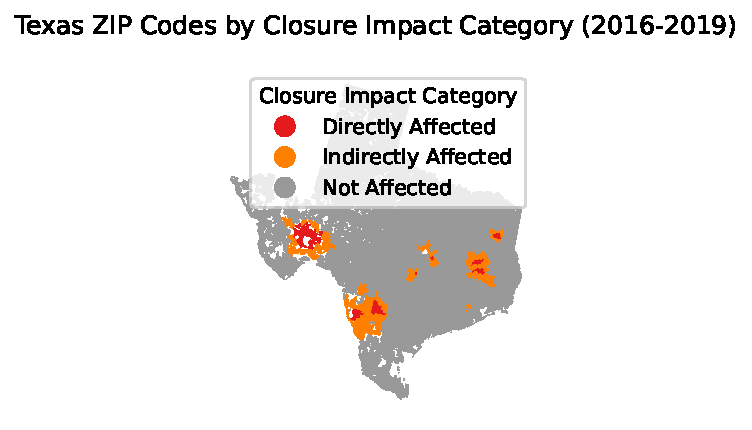
\includegraphics{Sujie- Abu Bakar_files/figure-pdf/cell-43-output-1.pdf}

\subsection{Reflecting on the exercise (10
pts)}\label{reflecting-on-the-exercise-10-pts}

\textbf{• (Partner 1) The ``first-pass'' method we're using to address
incorrectly identified closures in the data is imperfect. Can you think
of some potential issues that could arise still and ways to do a better
job at confirming hospital closures?}

\textbf{The limitations and issues about current approach are:} Delayed
reopenings. If a hospital closes but reopens later under a different
name or management, it may still be incorrectly counted as a closure.
This problem is common in facilities that undergo temporary closures for
renovations or changes in ownership.

The closure detection focuses only on the termination status without
considering geographical factors. In rural areas, where hospital
coverage is sparse, a closure has a more significant impact on access
than it might be in an urban setting with multiple nearby hospitals.

Data completeness and consistency. Hospital data may not be consistently
reported or may have gaps due to issues in data collection or reporting
delays. This could lead to misidentification if a hospital simply fails
to report data in one year but resumes the next year.

Mergers and new names-- Hospitals might seem closed due to changes in
their certification number or mergers. They may still be active under a
different identity and potentially leading to incorrect closure
identification.

\textbf{Potential Improvements:} Data collection procedures can be
improved to ensure that mergers, rebranding and any type of changes are
properly reflected. Track name and address changes by developing a more
robust matching system that accounts for slight changes in hospital
names or addresses. Using similarity metrics can help identify hospitals
with minor name changes that might indicate the same facility under new
management.

Consider factors which can indicate the impact of closures

Geographical impact of closures is also important. For example, the
closure of the only hospital within a 20-mile radius has a different
implication than a closure in a well-served urban area. Therefore, it
could be interesting to analyze the geographical impact on surrounding
ZIP codes or regions.

\textbf{• (Partner 2) Consider the way we are identifying zip codes
affected by closures. How well does this reflect changes in
zip-code-level access to hospitals? Can you think of some ways to
improve this measure?}

The method assumes that if a zip code is in proximity of a hospital has
acces to the hospital without consodering accessibility and
accessibility infrastructure. To access a facility, the ZIP codes within
a 10-mile radius might be impacted by factors like road quality and
transportation. Every ZIP code area does not have a similar impact by a
closure. It could be interesting to conisder the demographic factors
such as age, income, and health impacted by a hospital closures.

Some ZIP codes may have access to alternative healthcare facilities,
such as urgent care centers and outpatient clinics, which can partially
mitigate the impact of hospital closures. However, areas without these
alternatives are more significantly affected.

Adding population and demographics data, weighting the impact of
closures by the population density and demographics of each affected ZIP
code could be more valuable. Identifying areas that lack alternative
healthcare facilities within a reasonable distance could be important.
Calculating averag, min and max travel times to the nearest operational
hospital can also be important.




\end{document}
